\documentclass{article}
\usepackage[utf8]{inputenc}
\usepackage[english,russian]{babel}
\usepackage{amsmath}
\usepackage{enumerate}
\usepackage[12pt]{extsizes}
\usepackage{xcolor,listings}
\usepackage[left=30mm, top=20mm, right=20mm, bottom=20mm, nohead, footskip=10mm]{geometry}


\usepackage[absolute,overlay]{textpos}
\usepackage{indentfirst}
\usepackage{float}
\restylefloat{table}
\usepackage{hyperref}
\usepackage{mathtext}
\usepackage{amsfonts}
\usepackage{amsthm}
\usepackage{tikz}
\usetikzlibrary{shapes,positioning,shadows,trees,automata,arrows.meta,shapes.geometric}
\usepackage{pgf-pie}
\usepackage{chngcntr}
\usepackage{pdfpages}
\usepackage{systeme}
\usepackage{empheq}
\usepackage{subcaption}
\numberwithin{equation}{section}
\counterwithout{figure}{section}

\pagestyle{plain}

\definecolor{String}{RGB}{134, 179, 0}
\definecolor{KeyColor}{RGB}{160,0,102}


\captionsetup[lstlisting]{
	singlelinecheck=false,
	margin=3pt,
	font=,skip=5pt,
	font={bf}
}

\lstdefinestyle{style}{
	aboveskip=0pt,
	belowskip=10pt,
	showspaces=false,
	showstringspaces=false,
	basicstyle=\ttfamily\footnotesize,
	numbers=left,
	% texcl=true,
	breaklines=true,
	postbreak=\mbox{\textcolor{red}{$\hookrightarrow$}\space},
	keywordstyle=\color{KeyColor},
	identifierstyle=\color{black},
	numberstyle=\scriptsize,
	stringstyle=\color{String},
	commentstyle=\color{gray},
	frame=tb
}

\begin{document}
    \thispagestyle{empty}
	\begin{center}
		Санкт-Петербургский политехнический университет Петра Великого\\
		Институт прикладной математики и механики\\
		Кафедра <<Телематика (при ЦНИИ РТК)>>\\
		\vspace*{\fill}
		\textbf{\Large{КУРСОВАЯ РАБОТА}}\\
		\vspace{0.5cm}
        \large{по дисциплине <<Семинар по роботизированным системам>>\\}
        \large{на тему <<Муравьиный алгоритм и алгоритм коллективного распределения целей>>}\\
        \vspace{1cm}
        по направлению 02.04.01.02 <<Организация и управление суперкомпьютерными системами>>
	\end{center}
	\vspace{3cm}
	\begin{tabular} {l l l}
	\hspace{10cm} & Выполнил: & Титов А.И.\\
	& Проверил: & Глазунов В.В.
	\end{tabular}
	\vspace*{\fill}
	\begin{center}
		Санкт-Петербург\\
		2019
    \end{center}
    \newpage


	\renewcommand\contentsname{Оглавление}
	\tableofcontents

	\newpage
	\addcontentsline{toc}{section}{ПОСТАНОВКА ЗАДАЧИ}
	\section*{ПОСТАНОВКА ЗАДАЧИ}

	Целью курсовой работы является реализация и исследование алгоритмов для построения оптимальных путей роботов до целей. Далее под роботом, для простоты, будет иметься в виду непосредственно начальная координата пути, а под целью, соответственно, конечная координата.

	Таким образом, требуется создать карту местности, на которой помещается набор роботов и набор целей, после чего каждому роботу оптимально назначить цель и построить путь до нее.

	Для этого требуется реализовать следующие алгоритмы:

    \begin{itemize}
        \item Алгоритм для процедурного построения реалистичной карты местности \cite{terrain};
        \item Алгоритм коллективного распределения целей \cite{plan};
        \item Алгоритм поиска пути \cite{path}.
	\end{itemize}

	Для генерации реалистичной карты среды выбран алгоритм Diamond-Square \cite{DS}. Алгоритм коллективного распределения целей описан в \cite{plan} в главе <<Алгоритм коллективного улучшения плана 3.7>> на стр. 102. Для вычисления пути от робота до цели рассматривается муравьиный алгоритм \cite{ant}.

	Выполняются следующие задачи для достижения цели:
	\begin{enumerate}
		\item Реализация алгоритма Diamond-Square;
		\item Реализация муравьиного алгоритма;
		\item Реализация алгоритма коллективного распределения целей;
		\item Исследования реализованного функционала.
	\end{enumerate}

	Реализация осуществляется на языке Python. Исследование реализованного функционала заключается в следующем:

	\begin{enumerate}
		\item Генерация 10 различных карт для каждого размера из: 25x25, 50x50, 100x100, 250x250, 500x500, 1000x1000;
		\item На каждой из сгенерированных карт создаются наборы роботов и, соответственно, цели к ним в численности: 5, 10, 20, 50 (наборов каждого размера для каждой карты тоже должно быть по 10, но из соображений производительности этот пункт опущен);
		\item Для заданных наборов распределяются цели по роботам;
		\item Для каждого построенного набора строятся графики, отображающие зависимость времени выполнения программы от размеров карт и численности роботов. (В изначальном задании указано построить график, содержащий все измеренные времена, но для наглядности графики строятся только для средних элементов замеров, а полную картину отражают таблицы в \hyperref[sec:time]{ПРИЛОЖЕНИЕ Б});
		\item Теоретическое исследование реализуемого функционала.
	\end{enumerate}

	\newpage
	\section{Описание алгоритмов}

		В данной главе представлен разбор теоретических принципов работы реализуемых алгоритмов.

		\subsection{Алгоритм Diamond-Square}

			В данной работе для процедурной генерации реалистичной карты местности используется алгоритм Diamond-Square\cite{DS}. Прочие применяемые алгоритмы описаны в \cite{terrain}.

			Алгоритм имеет ограничения на размеры получаемой карты высот - $(2^{n} + 1)\times(2^{n} + 1)$.

			\begin{figure}[H]
				\centering
				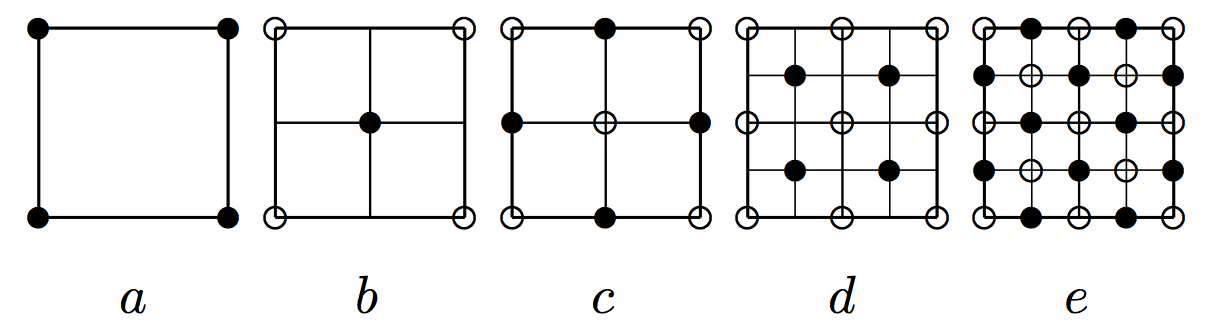
\includegraphics[width=\textwidth]{data/DS.png}
				\vspace{-0.5cm}
				\caption{Этапы работы алгоритма Diamond-Square}\label{fig:DS}
			\end{figure}

			Алгоритм включает в себя следующие этапы (отображены на \hyperref[fig:DS]{Рис. 1}):

			\begin{enumerate}[a)]
				\item \textbf{Инициализация}
					Пусть $n$ и $m$ - заданные ширина и высота требуемой карты высот. Чтобы использовать алгоритм для заданного размера требуется создать карту с шириной и высотой равными:
					\[ n' = 2^{\log_2 (max(n,m) - 1)} + 1 \]
					Для каждого углового элемента полученной карты генерируем случайное значение. Диапазон случайных значений в общем случае может быть любым, но в данной работе возьмем его равным $[0, \frac{n + m}{2}]$. В целом данный диапазон не влияет на производительность алгоритма или на возможность его реализации, он может быть и отрицательным, как, например в случае, когда 0 - это уровень моря.
				\item \textbf{Этап Diamond}
					На этом этапе находится центральная точка рассматриваемого квадрата, как среднее значение от его углов:
					\[ m[s/2][s/2] = \frac{m[0][0] + m[0][s] + m[s][0] + m[s][s]}{4} + \tau \]
					где $m$ - это рассматриваемый квадрат, $s$ - количество узлов на ребре квадрата. $\tau$ - случайная величина (шум), диапазон случайной величины $[-R * s, R * s]$, где $R$ - задаваемый коэффициент.
				\item \textbf{Этап Square}
					Здесь рассматривается ромб с вершинами, вычисленными на этапе Diamond. Подход схожий с этапом Diamond, только теперь высчитываются центральные элементы ребер квадрата по двум углам квадрата и двум центральным точкам, одна из которых - центр рассматриваемого квадрата, а вторая центр соседствующего квадрата. Существует проблема на краях генерируемой карты, ведь в таком случае нет центра соседствующего квадрата. В данной работе было принято следующее решение: при отсутствии соседствующего квадрата брать среднее от 3-ех точек - двух вершин и центра рассматриваемого квадрата.
				\item[d-e)] \textbf{Итерации по рассматриваемым квадратам}
					Итерации проходят по строкам и столбцам с шагом $s$:\\
					В каждой итерации по столбцам происходят этапы Square и Diamond, если итерация упирается в край карты, то происходит переход на следующую строку. При достижении правого нижнего угла матрицы значение $s$ обновляется $s = s / 2$ и итерации по строкам и столбцам происходят заново.\\
					Критерий останова: $s = 2$.
			\end{enumerate}

			После выполнения приведенных выше этапов построенная карта обрезается до размера $n \times m$.

		\subsection{Муравьиный алгоритм}

			Для построения путей роботов до целей был выбран муравьиный алгоритм \cite{ant}. Алгоритм имеет хорошую практическую применимость в такого рода задачах \cite{ant}\cite{ant1}\cite{ant2}. Существуют и прочие алгоритмы, которые весьма подробно описаны в \cite{path}.

			Основная идея алгоритма заключается в следующем:\\ Запустить на карту некоторую популяцию муравьев, которые должны дойти от начальной точки до конечной, при том каждую вершину пути муравей выбирает основываясь на концентрации феромона на вершине. После того, как все муравьи построили путь - они обновляют концентрацию феромона для каждой вершины, которая была задействована в построении пути. Далее запускается следующая популяция муравьев, которая основывается на уже обновленных значениях концентрации феромона.

			Данный алгоритм имеет низкую производительность при использовании его в чистом виде, однако при применении эвристик можно добиться значительного улучшения производительности.

			Основные этапы реализуемого муравьиного алгоритма:
			\begin{itemize}
				\item Изначально генерируется матрица, содержащая значения концентрации феромонов $\tau_{ij}$  . Для простоты матрица заполняется случайными очень маленькими значениями (в общем случае изначально значения должны быть равными 0).
			\end{itemize}
		\subsection{Алгоритм коллективного распределения целей}

    \newpage
	\section{Программная реализация}

	\newpage
	\section{Результаты}

		\subsection{Diamond-Square}

			\begin{figure}[H]
				\centering
				\vspace{-0.5cm}
				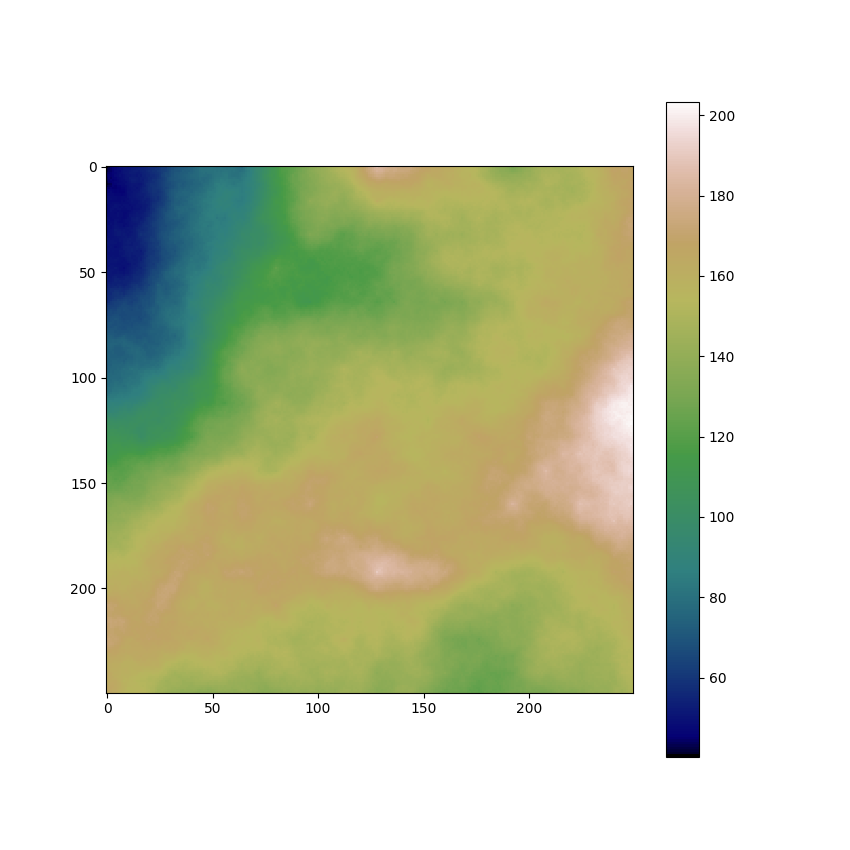
\includegraphics[width=0.6\textwidth]{data/maps_example/250x250.png}
				\vspace{-0.5cm}
				\caption{Карта размера 250x250}\label{fig:map1}
			\end{figure}

			\begin{figure}[H]
				\centering
				\vspace{-0.5cm}
				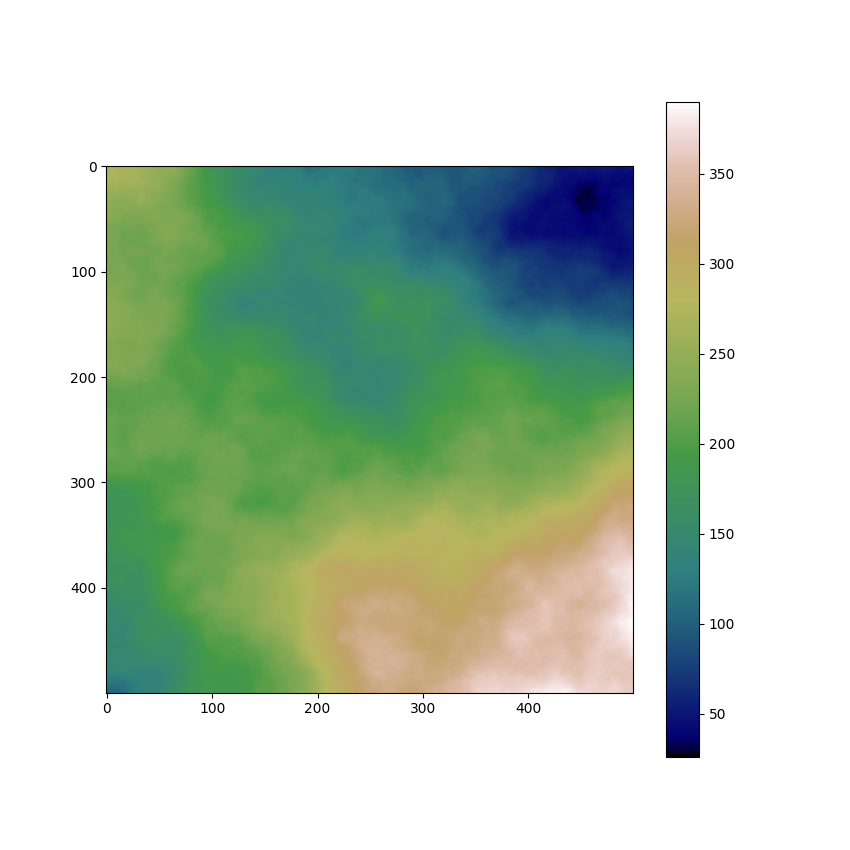
\includegraphics[width=0.6\textwidth]{data/maps_example/500x500.png}
				\vspace{-0.5cm}
				\caption{Карта размера 500x500}\label{fig:map2}
			\end{figure}

		\subsection{Муравьиный алгоритм}

			\begin{figure}[H]
				\vspace{-0.5cm}
				\centering
				\begin{subfigure}[b]{0.49\textwidth}
					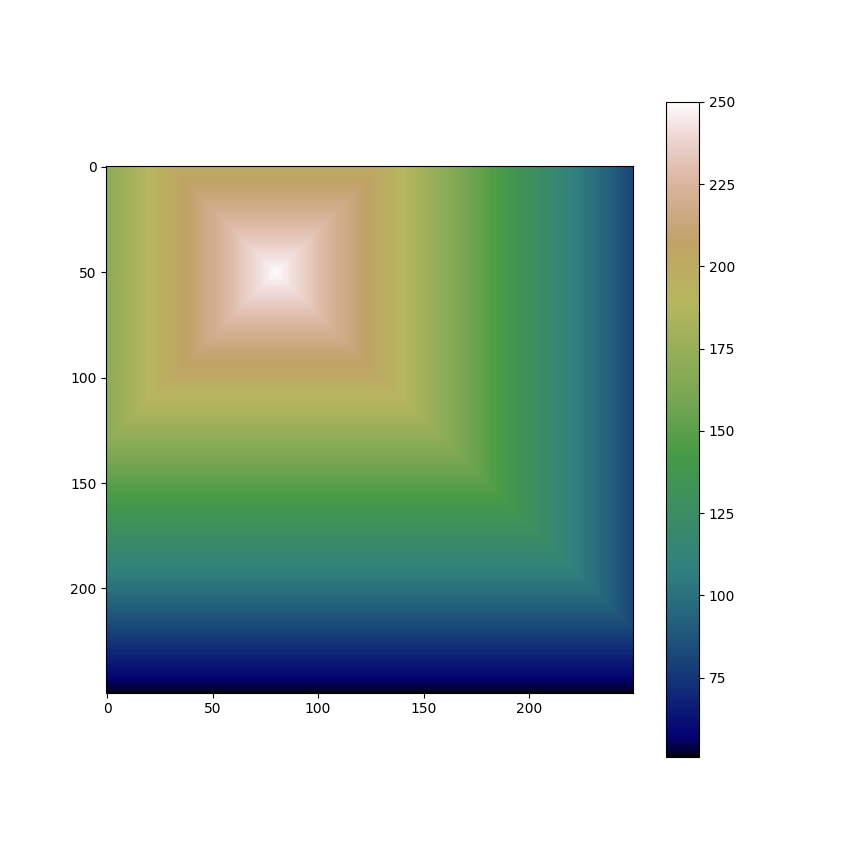
\includegraphics[width=\textwidth]{data/heuristics_example/heuristic_d_250x250.png}
					\caption*{Карта 250x250, Цель (50, 80)}
				\end{subfigure}
				\begin{subfigure}[b]{0.49\textwidth}
					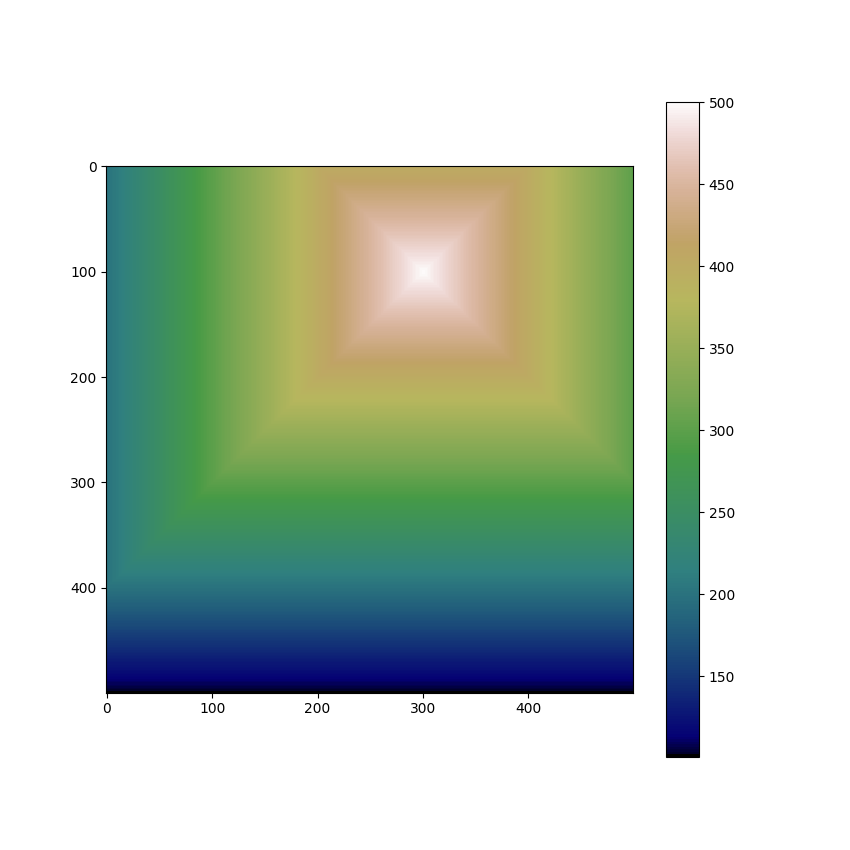
\includegraphics[width=\textwidth]{data/heuristics_example/heuristic_d_500x500.png}
					\caption*{Карта 500x500, Цель (345, 345)}
				\end{subfigure}
				\caption{Эвристики по расстоянию}\label{fig:heur_d}
			\end{figure}

			\begin{figure}[H]
				\vspace{-0.5cm}
				\centering
				\begin{subfigure}[b]{0.49\textwidth}
					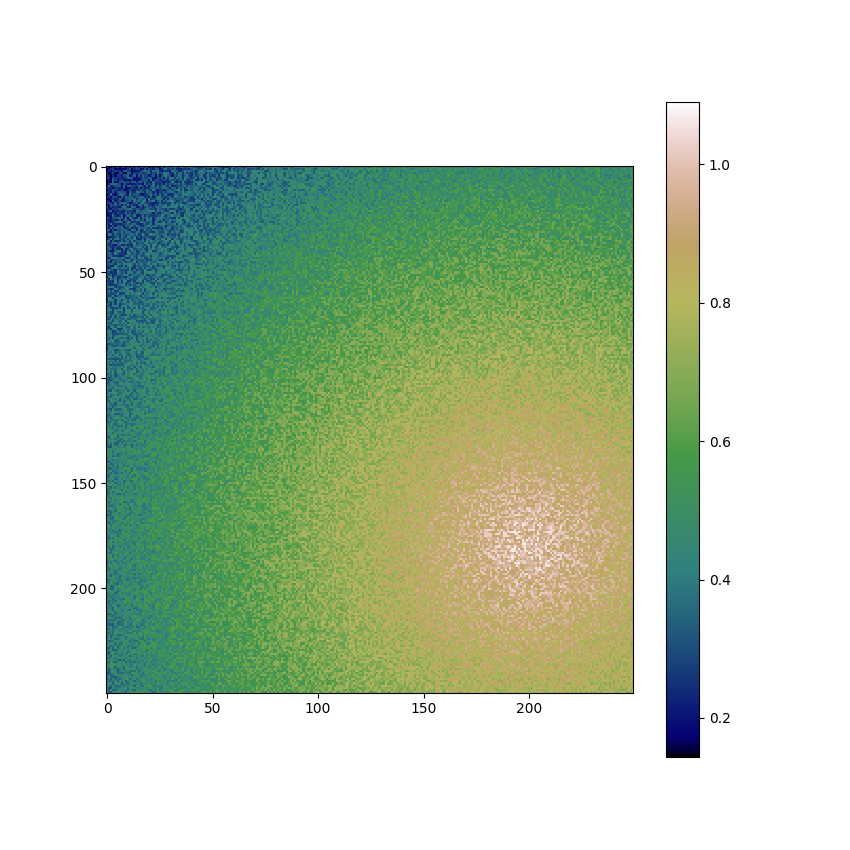
\includegraphics[width=\textwidth]{data/heuristics_example/pheromone_250x250.png}
					\caption*{Карта 250x250, Цель (50, 80)}
				\end{subfigure}
				\begin{subfigure}[b]{0.49\textwidth}
					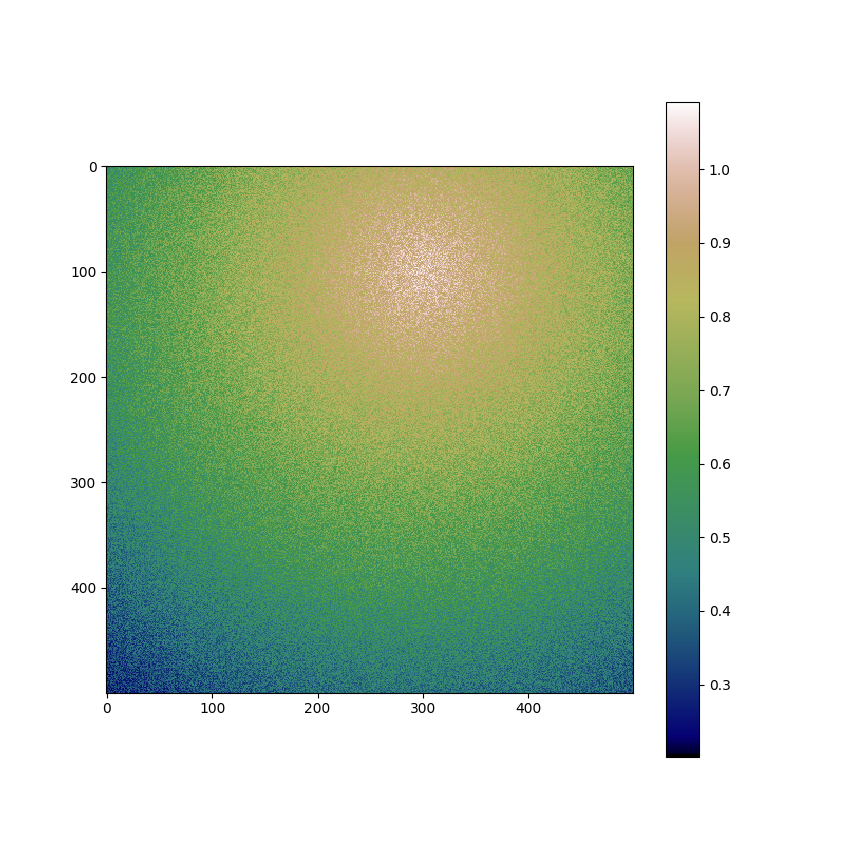
\includegraphics[width=\textwidth]{data/heuristics_example/pheromone_500x500.png}
					\caption*{Карта 500x500, Цель (345, 345)}
				\end{subfigure}
				\caption{Начальная концентрация феромонов}\label{fig:pher}
			\end{figure}

			\begin{figure}[H]
				\centering
				\vspace{-0.5cm}
				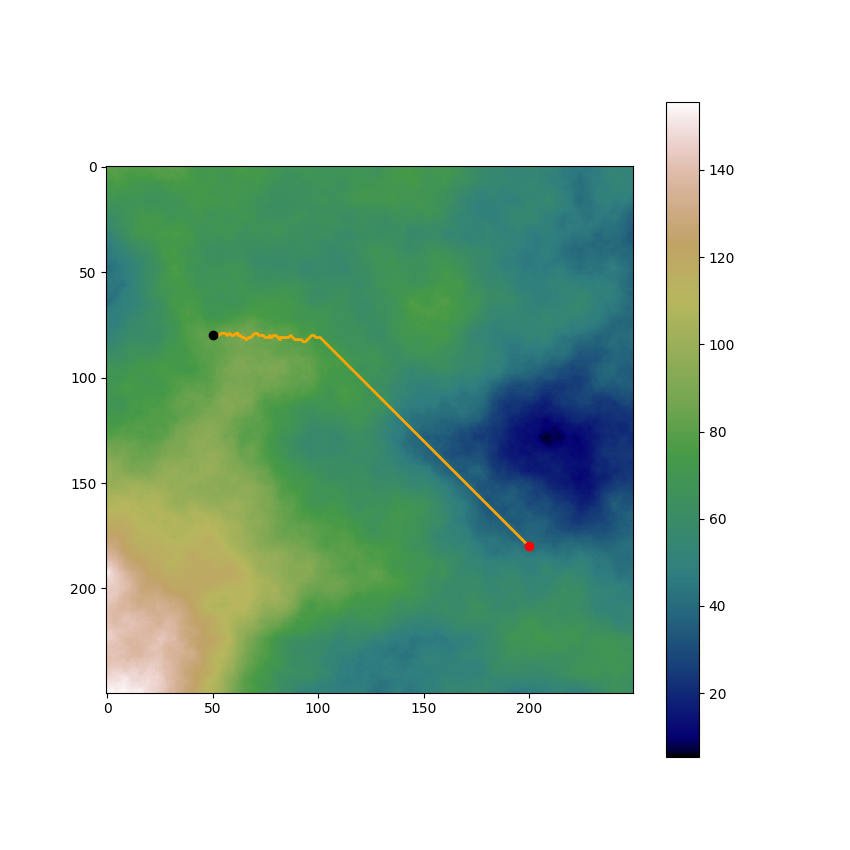
\includegraphics[width=0.6\textwidth]{data/path_example/250x250.png}
				\vspace{-0.5cm}
				\caption{Построенный путь для робота на карте размера 250x250}\label{fig:rob1}
			\end{figure}

			\begin{figure}[H]
				\centering
				\vspace{-0.5cm}
				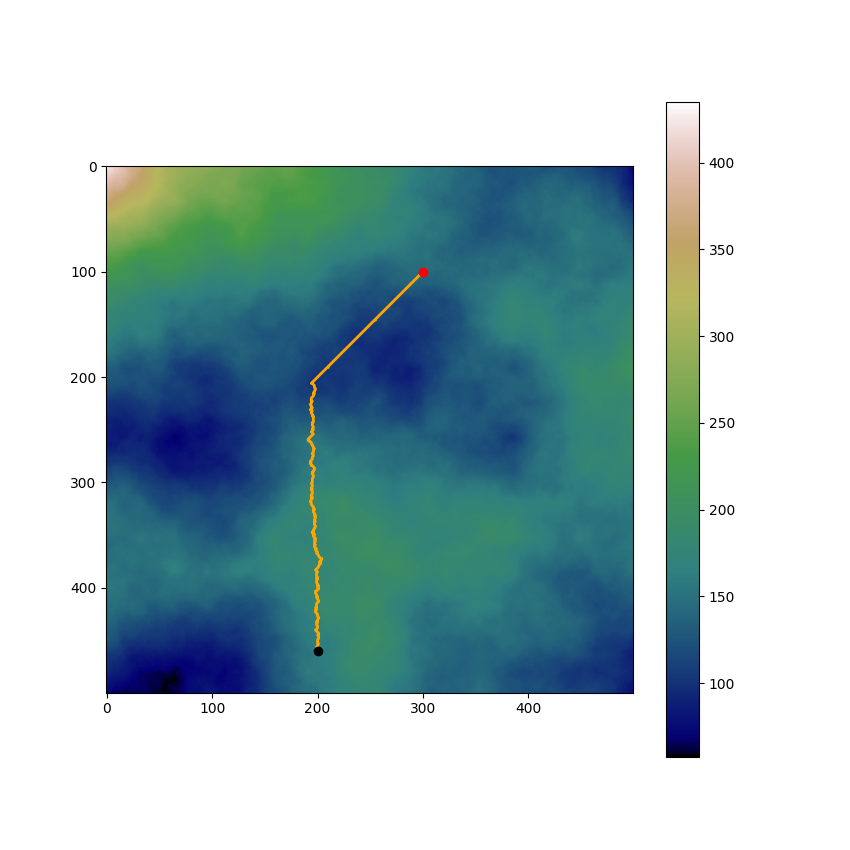
\includegraphics[width=0.6\textwidth]{data/path_example/500x500.png}
				\vspace{-0.5cm}
				\caption{Построенный путь для робота на карте размера 500x500}\label{fig:rob2}
			\end{figure}

		\subsection{Коллективное распределение целей}

			\begin{figure}[H]
				\centering
				\vspace{-0.5cm}
				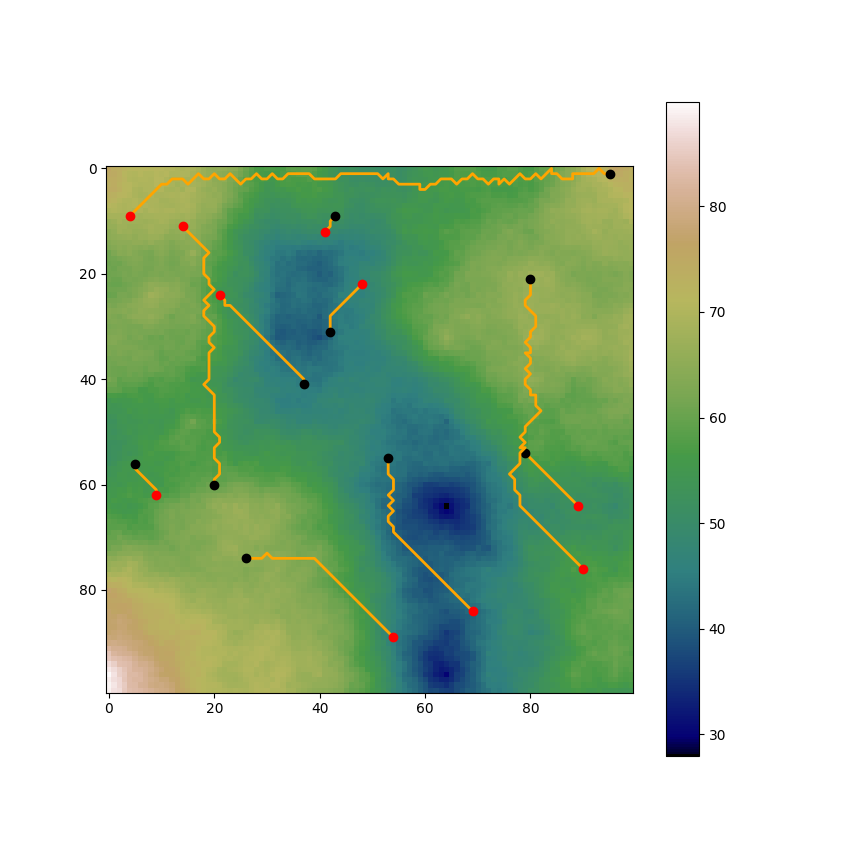
\includegraphics[width=0.6\textwidth]{data/mean_paths/100x100/10.png}
				\vspace{-0.5cm}
				\caption{Построенные пути для 10 роботов на карте размера 100x100}\label{fig:5robs}
			\end{figure}

			\begin{figure}[H]
				\centering
				\vspace{-0.5cm}
				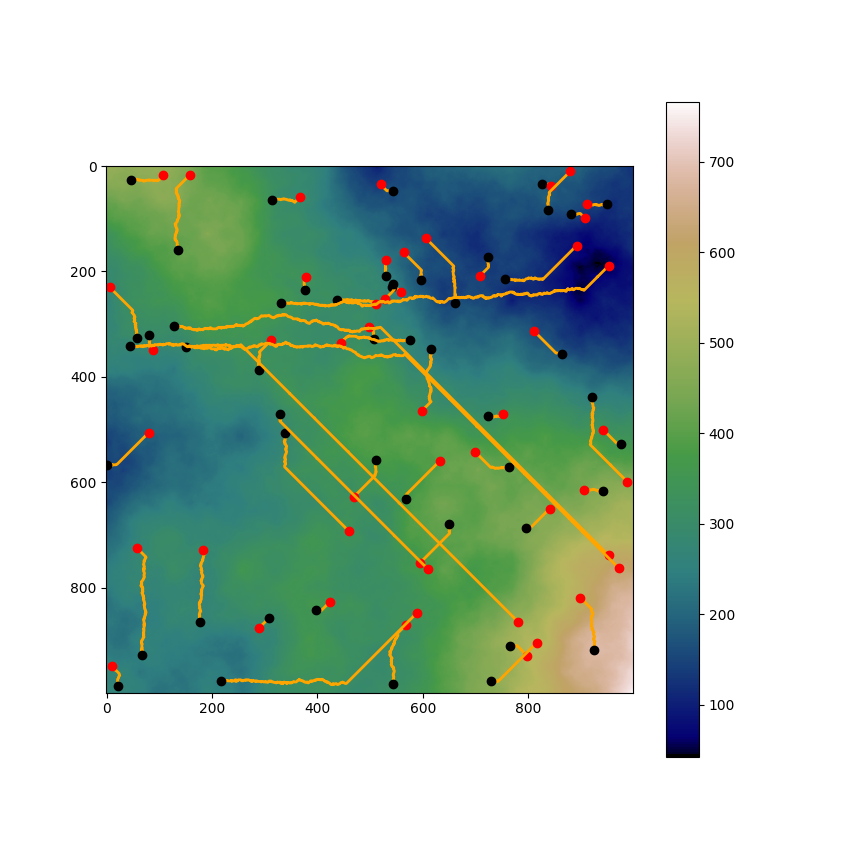
\includegraphics[width=0.6\textwidth]{data/mean_paths/1000x1000/50.png}
				\vspace{-0.5cm}
				\caption{Построенные пути для 50 роботов на карте размера 1000x1000}\label{fig:50robs}
			\end{figure}

		\subsection{Замеры времени работы}

			\begin{figure}[H]
				\centering
				\vspace{-0.5cm}
				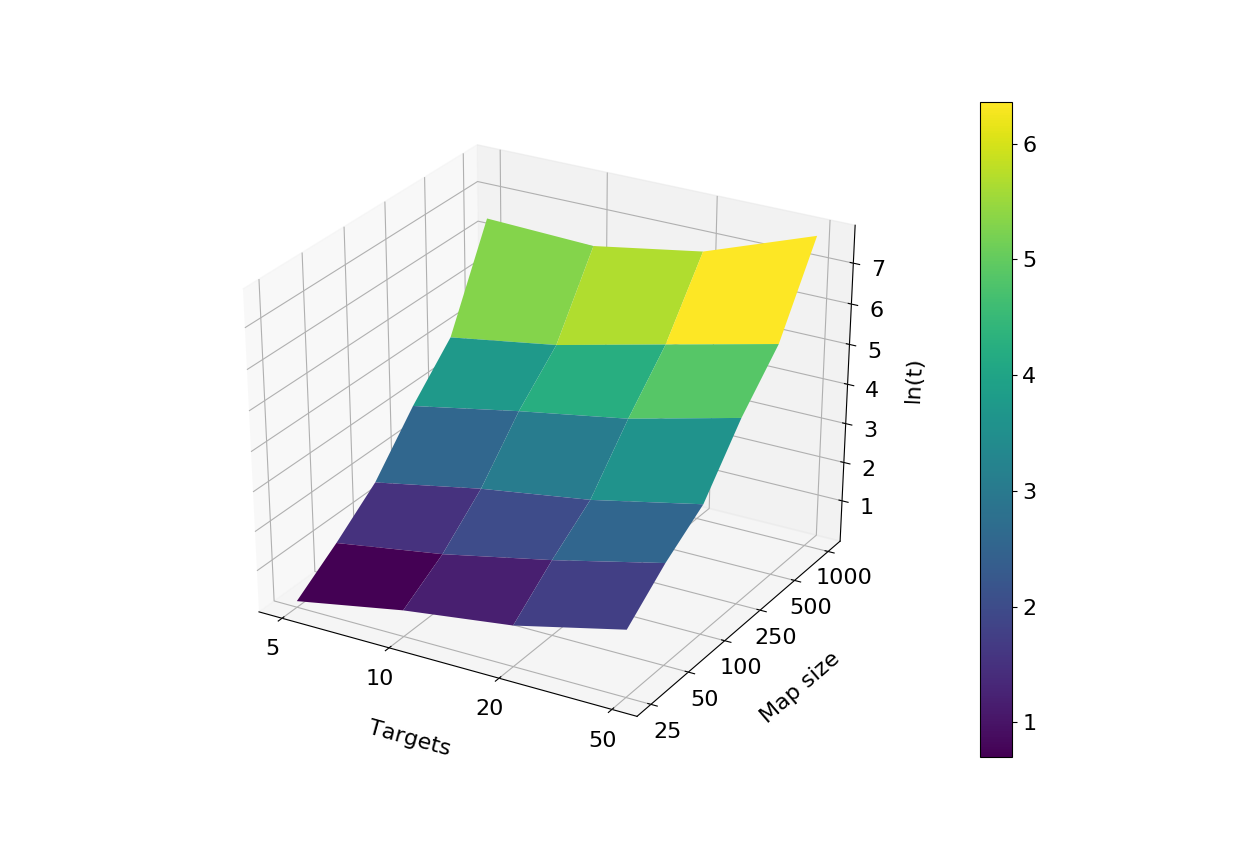
\includegraphics[width=\textwidth]{data/mean_surface.png}
				\vspace{-0.5cm}
				\caption{Зависимость времени вычислений (с.) от размера карты и количества роботов}\label{fig:time_surface}
			\end{figure}

    \newpage
    \addcontentsline{toc}{section}{ЗАКЛЮЧЕНИЕ}
    \section*{ЗАКЛЮЧЕНИЕ}

    \newpage
	\renewcommand\refname{ЛИТЕРАТУРА}
	\addcontentsline{toc}{section}{ЛИТЕРАТУРА}
	\begin{thebibliography}{}
		\bibitem{terrain} Miguel Monteiro de Sousa Frade. Genetic Terrain Programming // Universidad de Extremadura, 2008, pp. 103
		\bibitem{plan} Каляев И.А. Модели и алгоритмы коллективного управления в группах роботов // Физматлит, 2009, 279с.
		\bibitem{path} Gregor Klančar. Path Planning // Wheeled Mobile Robotics, 2017, pp. 161-206
		\bibitem{DS} Jacob Olsen. Realtime Procedural Terrain Generation // University of Southern Denmark, 2004, pp. 20
		\bibitem{ant} M. Brand, M. Masuda, N. Wehner, X.-H. Yu. Ant colony optimization algorithm for robot path planning // Computer Design and Applications (ICCDA) 2010 International Conference on, vol. 3, 2010, pp. 436-440.
		\bibitem{ant1} Alpa Reshamwala, Deepika P Vinchurkar. Robot Path Planning using An Ant Colony Optimization Approach: A Survey // (IJARAI) International Journal of Advanced Research in Artificial Intelligence, Vol. 2, No.3, 2013, pp. 7
		\bibitem{ant2} Sangita Sarangi. Optimization of Robot Motion Planning using Ant Colony Optimization // National Institute of Technology, Rourkela, 2011, pp. 81
	\end{thebibliography}


    \newpage
    \addcontentsline{toc}{section}{ПРИЛОЖЕНИЕ А. Исходный код}
	\section*{ПРИЛОЖЕНИЕ А. Исходный код} \label{sec:code}
	Ниже приведен исходный код на языке Python
	\lstinputlisting[language = python, style=style, title={main.py}]{data/code/main.py}
	\lstinputlisting[language = python, style=style, title={graph.py}]{data/code/graph.py}
	\lstinputlisting[language = python, style=style, title={ant.py}]{data/code/ant.py}
	\lstinputlisting[language = python, style=style, title={planning.py}]{data/code/planning.py}
	\lstinputlisting[language = python, style=style, title={tools.py}]{data/code/tools.py}


    \newpage
    \addcontentsline{toc}{section}{ПРИЛОЖЕНИЕ Б. Таблицы замеров времени}
	\section*{ПРИЛОЖЕНИЕ Б. Таблицы замеров времени} \label{sec:time}
	Ниже приведены замеры времени (c.) муравьиного алгоритма для каждой сгенерированной карты и каждого количества роботов:

	\begin{table}[H]
\centering
\begin{tabular}{|r|l|l|l|l|}
\hline
№ карты\textbackslash Кол-во роботов & \textbf{5} & \textbf{10} & \textbf{20} & \textbf{50}\\ \hline
1 & 0.0 & 0.0 & 0.0 & 0.004\\ \hline
2 & 0.0 & 0.0 & 0.001 & 0.004\\ \hline
3 & 0.0 & 0.0 & 0.0 & 0.005\\ \hline
4 & 0.0 & 0.0 & 0.001 & 0.003\\ \hline
5 & 0.0 & 0.0 & 0.0 & 0.004\\ \hline
6 & 0.0 & 0.0 & 0.0 & 0.004\\ \hline
7 & 0.0 & 0.0 & 0.0 & 0.004\\ \hline
8 & 0.0 & 0.0 & 0.0 & 0.004\\ \hline
9 & 0.0 & 0.0 & 0.0 & 0.004\\ \hline
10 & 0.0 & 0.0 & 0.0 & 0.005\\ \hline
Средний элемент & 0.0 & 0.0 & 0.0 & 0.004\\ \hline
\end{tabular}
\caption*{Размер карты: 25x25}
\end{table}

	\begin{table}[H]
\centering
\begin{tabular}{|r|l|l|l|l|}
\hline
№ карты\textbackslash Кол-во роботов & \textbf{5} & \textbf{10} & \textbf{20} & \textbf{50}\\ \hline
1 & 0.0 & 0.0 & 0.001 & 0.005\\ \hline
2 & 0.0 & 0.0 & 0.0 & 0.003\\ \hline
3 & 0.0 & 0.0 & 0.0 & 0.004\\ \hline
4 & 0.0 & 0.0 & 0.0 & 0.004\\ \hline
5 & 0.0 & 0.0 & 0.001 & 0.003\\ \hline
6 & 0.0 & 0.0 & 0.001 & 0.004\\ \hline
7 & 0.0 & 0.0 & 0.0 & 0.004\\ \hline
8 & 0.0 & 0.0 & 0.0 & 0.003\\ \hline
9 & 0.0 & 0.0 & 0.0 & 0.004\\ \hline
10 & 0.0 & 0.0 & 0.0 & 0.004\\ \hline
Средний элемент & 0.0 & 0.0 & 0.0 & 0.004\\ \hline
\end{tabular}
\caption*{Размер карты: 50x50}
\end{table}

	\begin{table}[H]
\centering
\begin{tabular}{|r|l|l|l|l|}
\hline
№ карты\textbackslash Кол-во роботов & \textbf{5} & \textbf{10} & \textbf{20} & \textbf{50}\\ \hline
1 & 6.32895 & 8.73452 & 14.94095 & 24.71504\\ \hline
2 & 5.26532 & 9.12678 & 13.68367 & 30.10719\\ \hline
3 & 4.87571 & 12.12137 & 14.66411 & 26.09427\\ \hline
4 & 5.98595 & 7.40209 & 12.80597 & 23.22383\\ \hline
5 & 3.94488 & 10.1101 & 17.56255 & 28.4082\\ \hline
6 & 7.12389 & 8.61739 & 13.43984 & 25.22285\\ \hline
7 & 5.36162 & 8.51896 & 13.89583 & 25.27979\\ \hline
8 & 5.02578 & 9.56457 & 11.74729 & 23.15173\\ \hline
9 & 5.34449 & 13.91983 & 14.71402 & 22.08825\\ \hline
10 & 6.81967 & 9.45882 & 17.0239 & 31.06226\\ \hline
Средний элемент & 5.34449 & 9.12678 & 13.89583 & 25.22285\\ \hline
\end{tabular}
\caption*{Размер карты: 100x100}
\end{table}

	\begin{table}[H]
\centering
\begin{tabular}{|r|l|l|l|l|}
\hline
№ карты\textbackslash Кол-во роботов & \textbf{5} & \textbf{10} & \textbf{20} & \textbf{50}\\ \hline
1 & 42.28 & 32.36 & 52.149 & 107.196\\ \hline
2 & 19.016 & 27.002 & 69.753 & 103.928\\ \hline
3 & 20.361 & 30.919 & 45.16 & 103.125\\ \hline
4 & 17.649 & 38.522 & 52.348 & 115.323\\ \hline
5 & 19.154 & 39.692 & 60.4 & 123.056\\ \hline
6 & 25.561 & 25.462 & 49.701 & 121.093\\ \hline
7 & 18.231 & 34.012 & 58.345 & 93.992\\ \hline
8 & 13.386 & 34.576 & 51.704 & 105.007\\ \hline
9 & 17.922 & 35.839 & 48.99 & 98.7\\ \hline
10 & 23.871 & 26.686 & 54.966 & 103.896\\ \hline
Средний элемент & 19.016 & 32.36 & 52.149 & 103.928\\ \hline
\end{tabular}
\caption*{Размер карты: 250x250}
\end{table}

	\begin{table}[H]
\centering
\begin{tabular}{|r|l|l|l|l|}
\hline
№ карты\textbackslash Кол-во роботов & \textbf{5} & \textbf{10} & \textbf{20} & \textbf{50}\\ \hline
1 & 47.88517 & 73.60561 & 137.27325 & 308.64456\\ \hline
2 & 48.11748 & 105.09704 & 167.23236 & 321.9515\\ \hline
3 & 64.0862 & 109.30441 & 143.13767 & 335.52867\\ \hline
4 & 59.32068 & 187.01288 & 168.12613 & 364.50322\\ \hline
5 & 75.32691 & 124.74065 & 178.59087 & 319.94925\\ \hline
6 & 61.19254 & 79.99268 & 128.15281 & 503.20078\\ \hline
7 & 51.79195 & 87.23905 & 198.67009 & 341.6798\\ \hline
8 & 58.80499 & 87.76271 & 282.89796 & 311.80583\\ \hline
9 & 56.37451 & 80.41181 & 277.18092 & 283.16109\\ \hline
10 & 56.46719 & 103.25168 & 243.64185 & 409.125\\ \hline
Средний элемент & 56.46719 & 87.76271 & 168.12613 & 321.9515\\ \hline
\end{tabular}
\caption*{Размер карты: 500x500}
\end{table}

	\begin{table}[H]
\centering
\begin{tabular}{|r|l|l|l|l|}
\hline
№ карты\textbackslash Кол-во роботов & \textbf{5} & \textbf{10} & \textbf{20} & \textbf{50}\\ \hline
1 & 985.467 & 292.7 & 847.499 & 2510.479\\ \hline
2 & 289.546 & 551.286 & 879.198 & 1478.341\\ \hline
3 & 775.556 & 516.55 & 493.118 & 2206.797\\ \hline
4 & 612.462 & 1196.722 & 596.369 & 2167.358\\ \hline
5 & 356.076 & 626.026 & 757.651 & 2049.006\\ \hline
6 & 258.133 & 1190.344 & 1356.154 & 2417.786\\ \hline
7 & 1100.106 & 554.877 & 1412.945 & 2335.377\\ \hline
8 & 715.701 & 372.302 & 1571.88 & 4075.243\\ \hline
9 & 905.145 & 777.733 & 2050.21 & 4158.513\\ \hline
10 & 170.516 & 1581.04 & 2182.638 & 4512.163\\ \hline
Средний элемент & 612.462 & 554.877 & 879.198 & 2335.377\\ \hline
\end{tabular}
\caption*{Размер карты: 1000x1000}
\end{table}


	Ниже приведены замеры времени (c.) алгоритма планирования для каждой сгенерированной карты и каждого количества роботов:

	\begin{table}[H]
\centering
\begin{tabular}{|r|l|l|l|l|}
\hline
№ карты\textbackslash Кол-во роботов & \textbf{5} & \textbf{10} & \textbf{20} & \textbf{50}\\ \hline
1 & 0.0 & 0.0 & 0.0 & 0.004\\ \hline
2 & 0.0 & 0.0 & 0.001 & 0.004\\ \hline
3 & 0.0 & 0.0 & 0.0 & 0.005\\ \hline
4 & 0.0 & 0.0 & 0.001 & 0.003\\ \hline
5 & 0.0 & 0.0 & 0.0 & 0.004\\ \hline
6 & 0.0 & 0.0 & 0.0 & 0.004\\ \hline
7 & 0.0 & 0.0 & 0.0 & 0.004\\ \hline
8 & 0.0 & 0.0 & 0.0 & 0.004\\ \hline
9 & 0.0 & 0.0 & 0.0 & 0.004\\ \hline
10 & 0.0 & 0.0 & 0.0 & 0.005\\ \hline
Средний элемент & 0.0 & 0.0 & 0.0 & 0.004\\ \hline
\end{tabular}
\caption*{Размер карты: 25x25}
\end{table}

	\begin{table}[H]
\centering
\begin{tabular}{|r|l|l|l|l|}
\hline
№ карты\textbackslash Кол-во роботов & \textbf{5} & \textbf{10} & \textbf{20} & \textbf{50}\\ \hline
1 & 0.0 & 0.0 & 0.001 & 0.005\\ \hline
2 & 0.0 & 0.0 & 0.0 & 0.003\\ \hline
3 & 0.0 & 0.0 & 0.0 & 0.004\\ \hline
4 & 0.0 & 0.0 & 0.0 & 0.004\\ \hline
5 & 0.0 & 0.0 & 0.001 & 0.003\\ \hline
6 & 0.0 & 0.0 & 0.001 & 0.004\\ \hline
7 & 0.0 & 0.0 & 0.0 & 0.004\\ \hline
8 & 0.0 & 0.0 & 0.0 & 0.003\\ \hline
9 & 0.0 & 0.0 & 0.0 & 0.004\\ \hline
10 & 0.0 & 0.0 & 0.0 & 0.004\\ \hline
Средний элемент & 0.0 & 0.0 & 0.0 & 0.004\\ \hline
\end{tabular}
\caption*{Размер карты: 50x50}
\end{table}

	\begin{table}[H]
\centering
\begin{tabular}{|r|l|l|l|l|}
\hline
№ карты\textbackslash Кол-во роботов & \textbf{5} & \textbf{10} & \textbf{20} & \textbf{50}\\ \hline
1 & 6.32895 & 8.73452 & 14.94095 & 24.71504\\ \hline
2 & 5.26532 & 9.12678 & 13.68367 & 30.10719\\ \hline
3 & 4.87571 & 12.12137 & 14.66411 & 26.09427\\ \hline
4 & 5.98595 & 7.40209 & 12.80597 & 23.22383\\ \hline
5 & 3.94488 & 10.1101 & 17.56255 & 28.4082\\ \hline
6 & 7.12389 & 8.61739 & 13.43984 & 25.22285\\ \hline
7 & 5.36162 & 8.51896 & 13.89583 & 25.27979\\ \hline
8 & 5.02578 & 9.56457 & 11.74729 & 23.15173\\ \hline
9 & 5.34449 & 13.91983 & 14.71402 & 22.08825\\ \hline
10 & 6.81967 & 9.45882 & 17.0239 & 31.06226\\ \hline
Средний элемент & 5.34449 & 9.12678 & 13.89583 & 25.22285\\ \hline
\end{tabular}
\caption*{Размер карты: 100x100}
\end{table}

	\begin{table}[H]
\centering
\begin{tabular}{|r|l|l|l|l|}
\hline
№ карты\textbackslash Кол-во роботов & \textbf{5} & \textbf{10} & \textbf{20} & \textbf{50}\\ \hline
1 & 42.28 & 32.36 & 52.149 & 107.196\\ \hline
2 & 19.016 & 27.002 & 69.753 & 103.928\\ \hline
3 & 20.361 & 30.919 & 45.16 & 103.125\\ \hline
4 & 17.649 & 38.522 & 52.348 & 115.323\\ \hline
5 & 19.154 & 39.692 & 60.4 & 123.056\\ \hline
6 & 25.561 & 25.462 & 49.701 & 121.093\\ \hline
7 & 18.231 & 34.012 & 58.345 & 93.992\\ \hline
8 & 13.386 & 34.576 & 51.704 & 105.007\\ \hline
9 & 17.922 & 35.839 & 48.99 & 98.7\\ \hline
10 & 23.871 & 26.686 & 54.966 & 103.896\\ \hline
Средний элемент & 19.016 & 32.36 & 52.149 & 103.928\\ \hline
\end{tabular}
\caption*{Размер карты: 250x250}
\end{table}

	\begin{table}[H]
\centering
\begin{tabular}{|r|l|l|l|l|}
\hline
№ карты\textbackslash Кол-во роботов & \textbf{5} & \textbf{10} & \textbf{20} & \textbf{50}\\ \hline
1 & 47.88517 & 73.60561 & 137.27325 & 308.64456\\ \hline
2 & 48.11748 & 105.09704 & 167.23236 & 321.9515\\ \hline
3 & 64.0862 & 109.30441 & 143.13767 & 335.52867\\ \hline
4 & 59.32068 & 187.01288 & 168.12613 & 364.50322\\ \hline
5 & 75.32691 & 124.74065 & 178.59087 & 319.94925\\ \hline
6 & 61.19254 & 79.99268 & 128.15281 & 503.20078\\ \hline
7 & 51.79195 & 87.23905 & 198.67009 & 341.6798\\ \hline
8 & 58.80499 & 87.76271 & 282.89796 & 311.80583\\ \hline
9 & 56.37451 & 80.41181 & 277.18092 & 283.16109\\ \hline
10 & 56.46719 & 103.25168 & 243.64185 & 409.125\\ \hline
Средний элемент & 56.46719 & 87.76271 & 168.12613 & 321.9515\\ \hline
\end{tabular}
\caption*{Размер карты: 500x500}
\end{table}

	\begin{table}[H]
\centering
\begin{tabular}{|r|l|l|l|l|}
\hline
№ карты\textbackslash Кол-во роботов & \textbf{5} & \textbf{10} & \textbf{20} & \textbf{50}\\ \hline
1 & 985.467 & 292.7 & 847.499 & 2510.479\\ \hline
2 & 289.546 & 551.286 & 879.198 & 1478.341\\ \hline
3 & 775.556 & 516.55 & 493.118 & 2206.797\\ \hline
4 & 612.462 & 1196.722 & 596.369 & 2167.358\\ \hline
5 & 356.076 & 626.026 & 757.651 & 2049.006\\ \hline
6 & 258.133 & 1190.344 & 1356.154 & 2417.786\\ \hline
7 & 1100.106 & 554.877 & 1412.945 & 2335.377\\ \hline
8 & 715.701 & 372.302 & 1571.88 & 4075.243\\ \hline
9 & 905.145 & 777.733 & 2050.21 & 4158.513\\ \hline
10 & 170.516 & 1581.04 & 2182.638 & 4512.163\\ \hline
Средний элемент & 612.462 & 554.877 & 879.198 & 2335.377\\ \hline
\end{tabular}
\caption*{Размер карты: 1000x1000}
\end{table}


    \newpage
    \addcontentsline{toc}{section}{ПРИЛОЖЕНИЕ В. Графики решений}
	\section*{ПРИЛОЖЕНИЕ В. Графики решений} \label{sec:png}
	Ниже представлены построенные пути с средним временем выполнения для разного числа роботов и разных размеров матриц (черным отмечены роботы, красным - цели):
	\begin{table}[H]
		\begin{tabular}{c c}
			\begin{subfigure}{0.5\linewidth}
				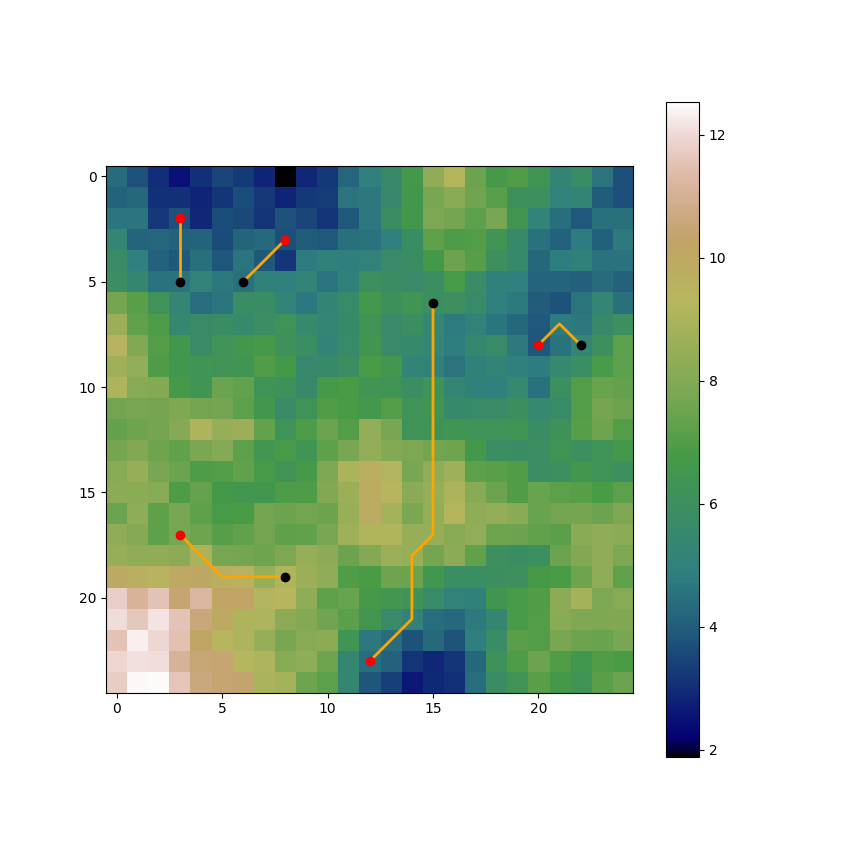
\includegraphics[width = 1.0\columnwidth]{data/mean_paths/25x25/5.png}
			\caption*{5 роботов}
			\end{subfigure}
			&
			\begin{subfigure}{0.5\linewidth}
				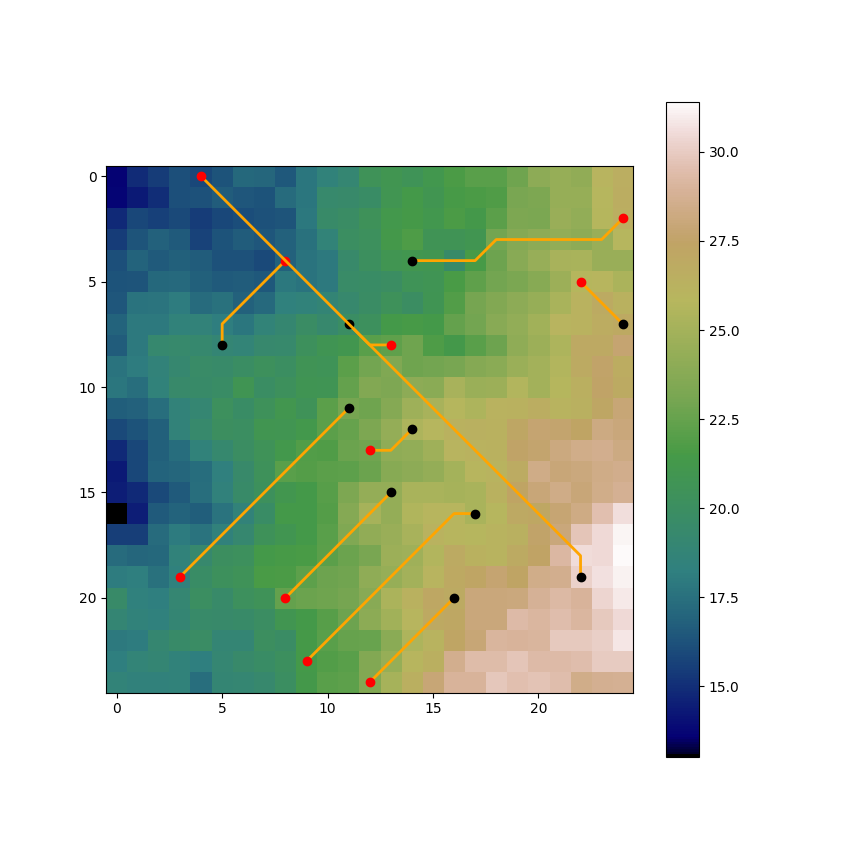
\includegraphics[width = 1.0\columnwidth]{data/mean_paths/25x25/10.png}
			\caption*{10 роботов}
			\end{subfigure}
			\\
            \begin{subfigure}{0.5\linewidth}
				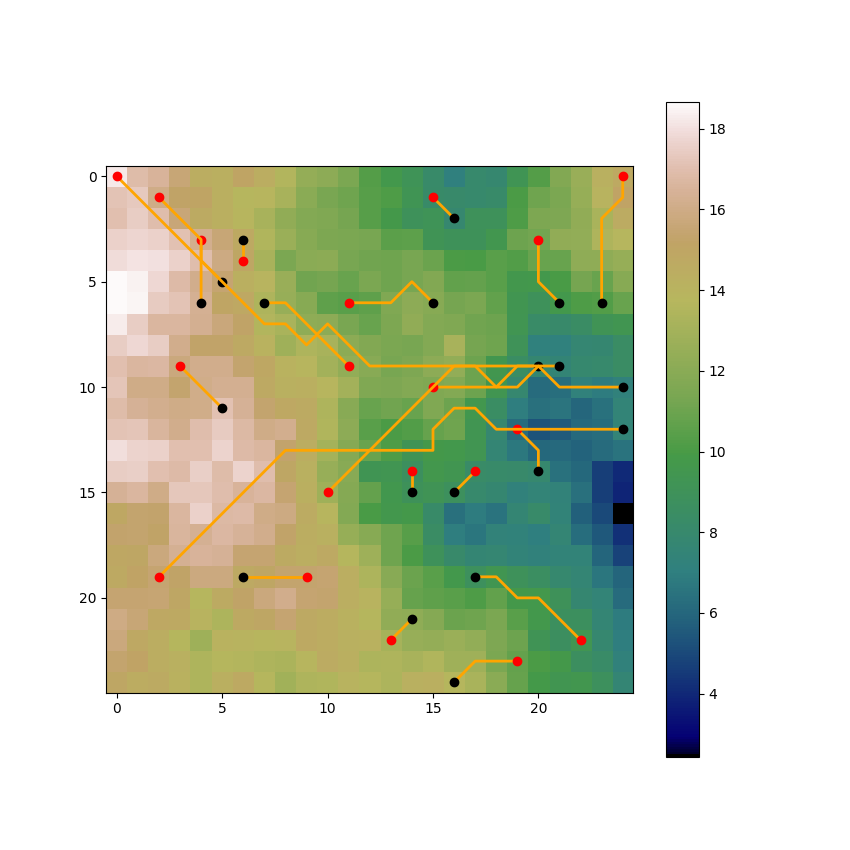
\includegraphics[width = 1.0\columnwidth]{data/mean_paths/25x25/20.png}
			\caption*{20 роботов}
			\end{subfigure}
			&
			\begin{subfigure}{0.5\linewidth}
				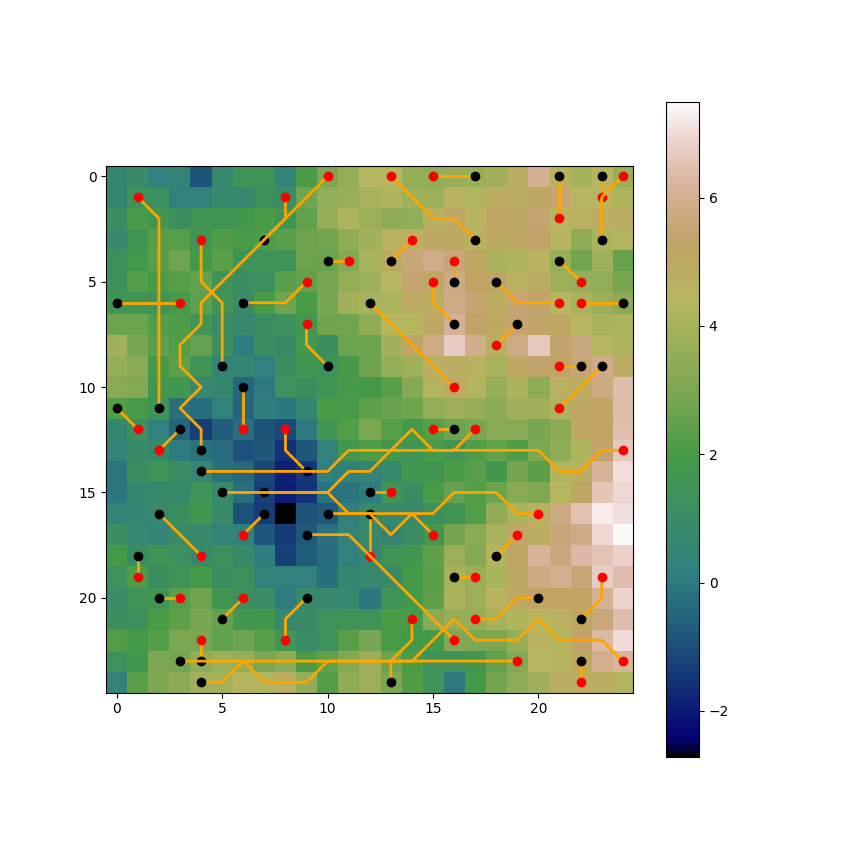
\includegraphics[width = 1.0\columnwidth]{data/mean_paths/25x25/50.png}
			\caption*{50 роботов}
			\end{subfigure}
        \end{tabular}
        \caption*{Размер карты: 25x25}
	\end{table}

	\begin{table}[H]
		\begin{tabular}{c c}
			\begin{subfigure}{0.5\linewidth}
				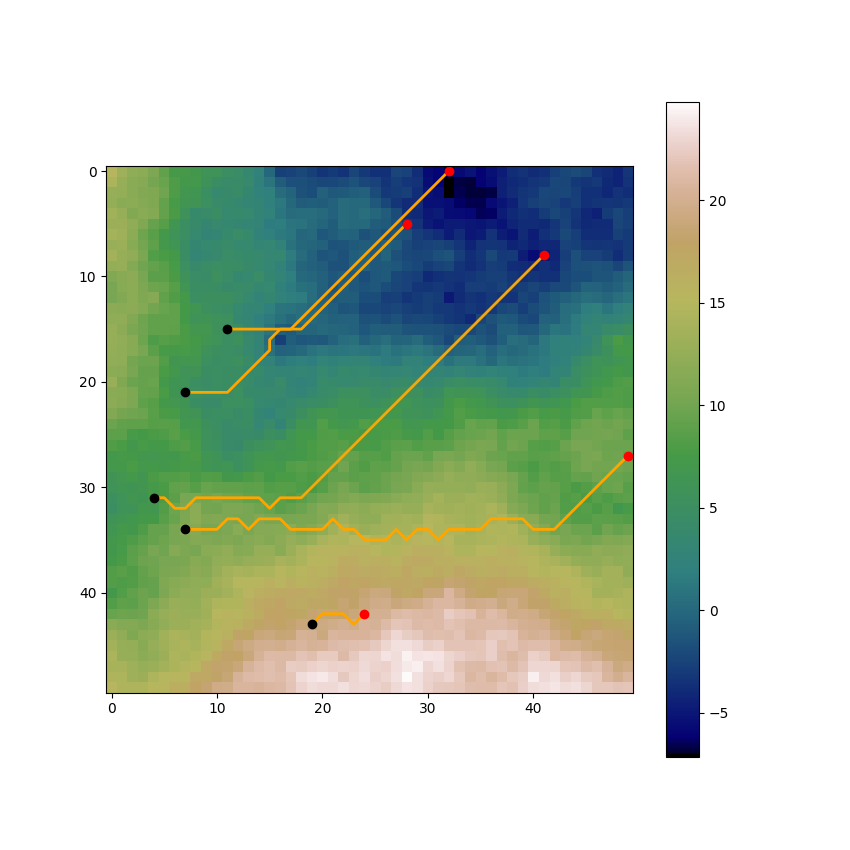
\includegraphics[width = 1.0\columnwidth]{data/mean_paths/50x50/5.png}
			\caption*{5 роботов}
			\end{subfigure}
			&
			\begin{subfigure}{0.5\linewidth}
				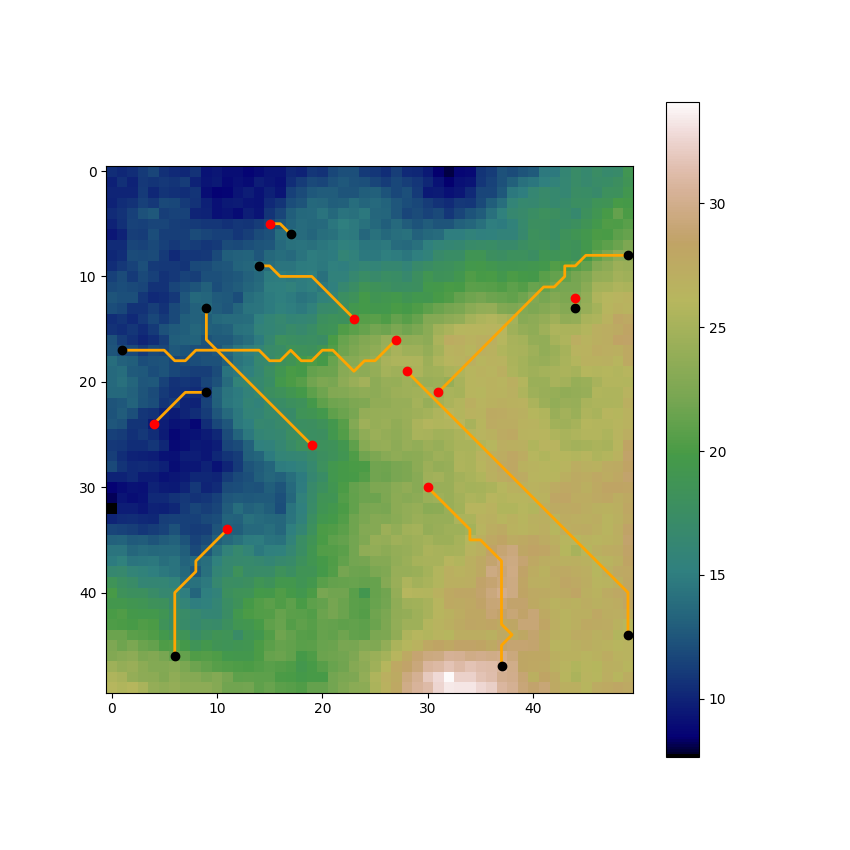
\includegraphics[width = 1.0\columnwidth]{data/mean_paths/50x50/10.png}
			\caption*{10 роботов}
			\end{subfigure}
			\\
            \begin{subfigure}{0.5\linewidth}
				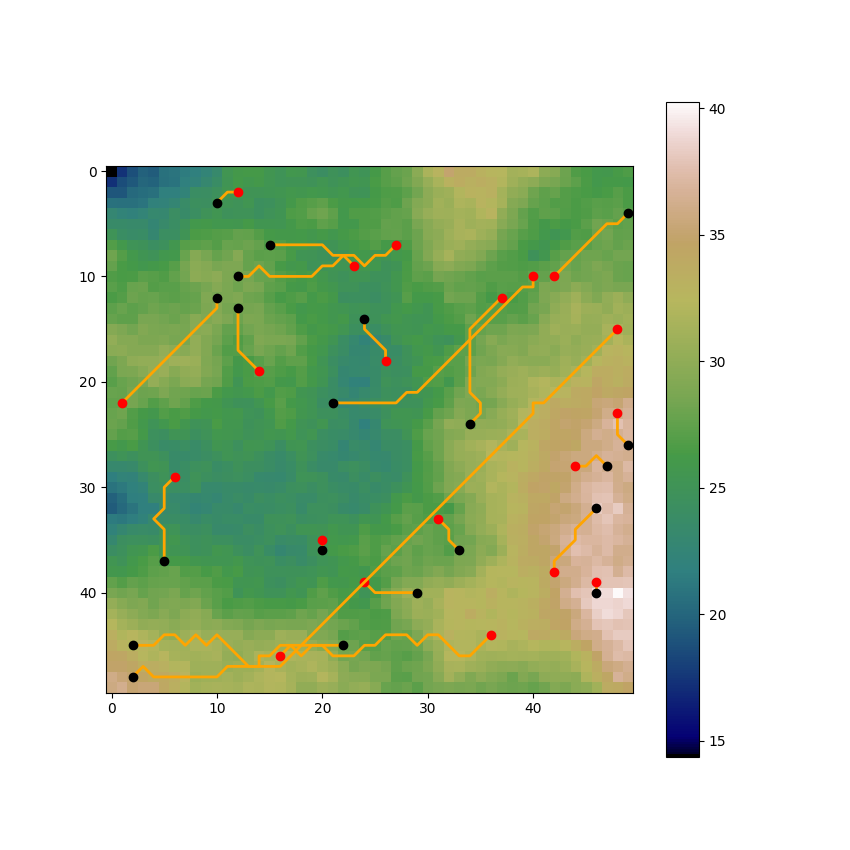
\includegraphics[width = 1.0\columnwidth]{data/mean_paths/50x50/20.png}
			\caption*{20 роботов}
			\end{subfigure}
			&
			\begin{subfigure}{0.5\linewidth}
				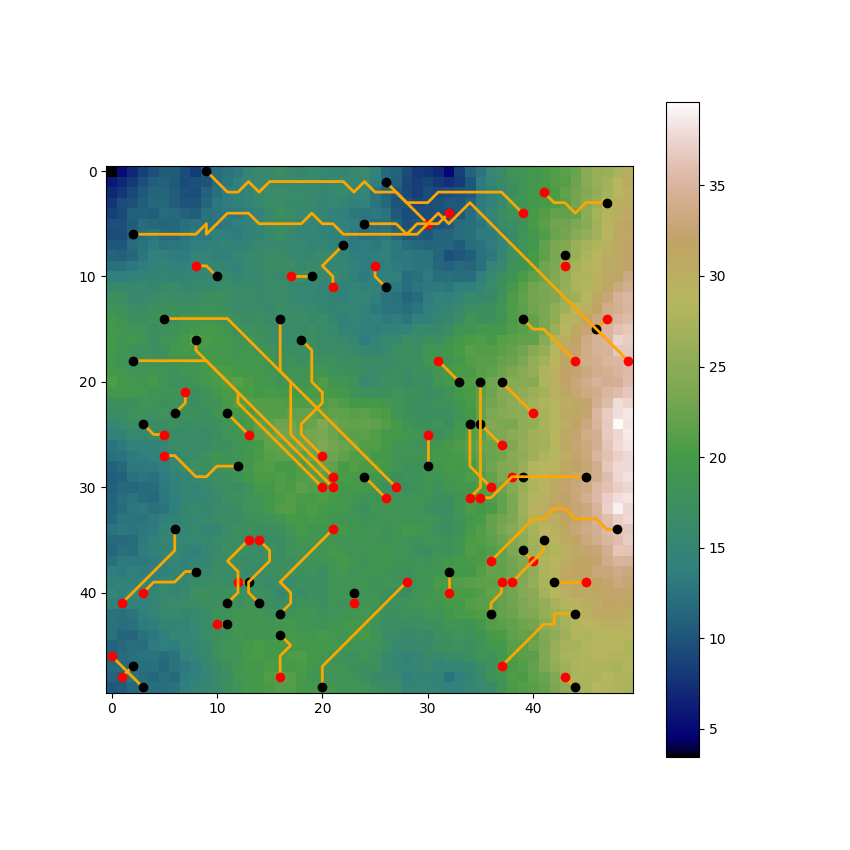
\includegraphics[width = 1.0\columnwidth]{data/mean_paths/50x50/50.png}
			\caption*{50 роботов}
			\end{subfigure}
        \end{tabular}
        \caption*{Размер карты: 50x50}
	\end{table}

	\begin{table}[H]
		\begin{tabular}{c c}
			\begin{subfigure}{0.5\linewidth}
				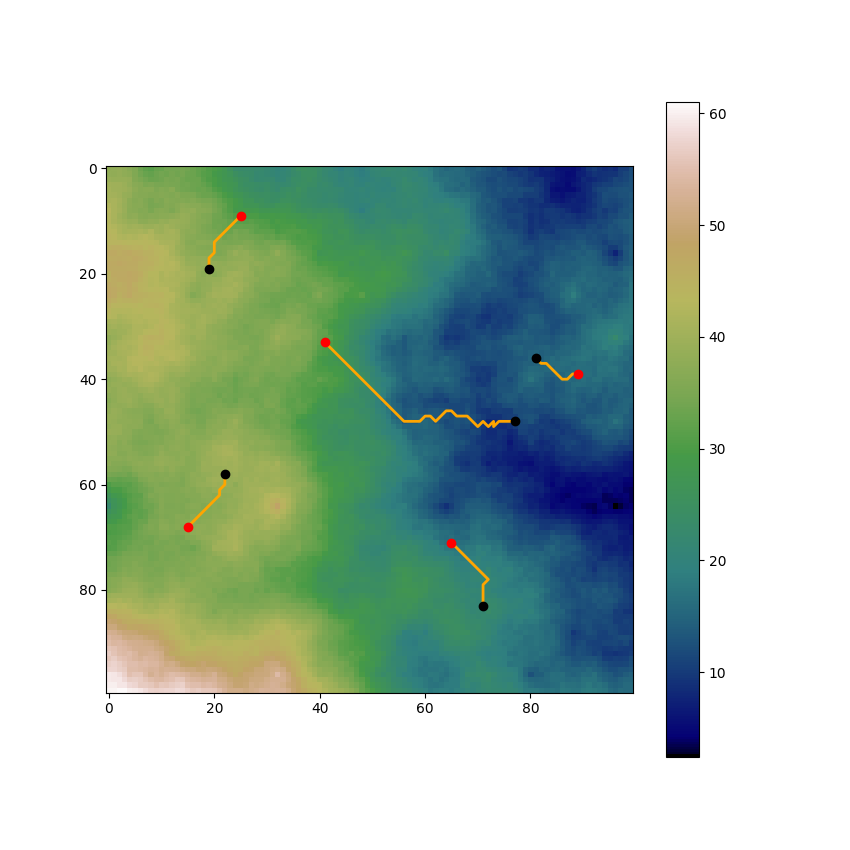
\includegraphics[width = 1.0\columnwidth]{data/mean_paths/100x100/5.png}
			\caption*{5 роботов}
			\end{subfigure}
			&
			\begin{subfigure}{0.5\linewidth}
				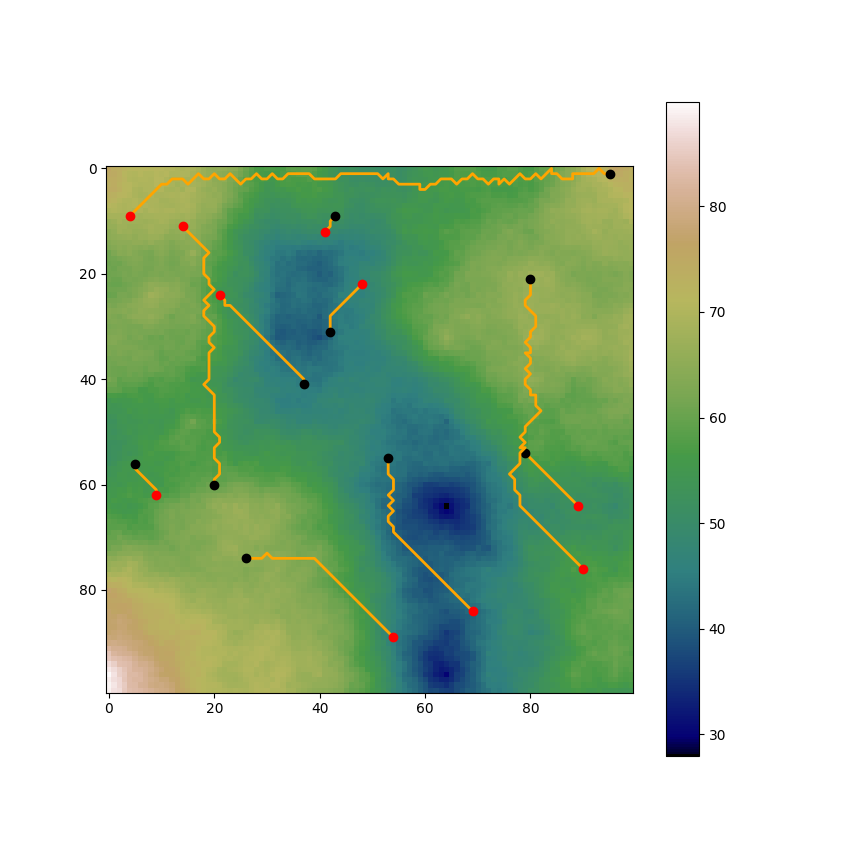
\includegraphics[width = 1.0\columnwidth]{data/mean_paths/100x100/10.png}
			\caption*{10 роботов}
			\end{subfigure}
			\\
            \begin{subfigure}{0.5\linewidth}
				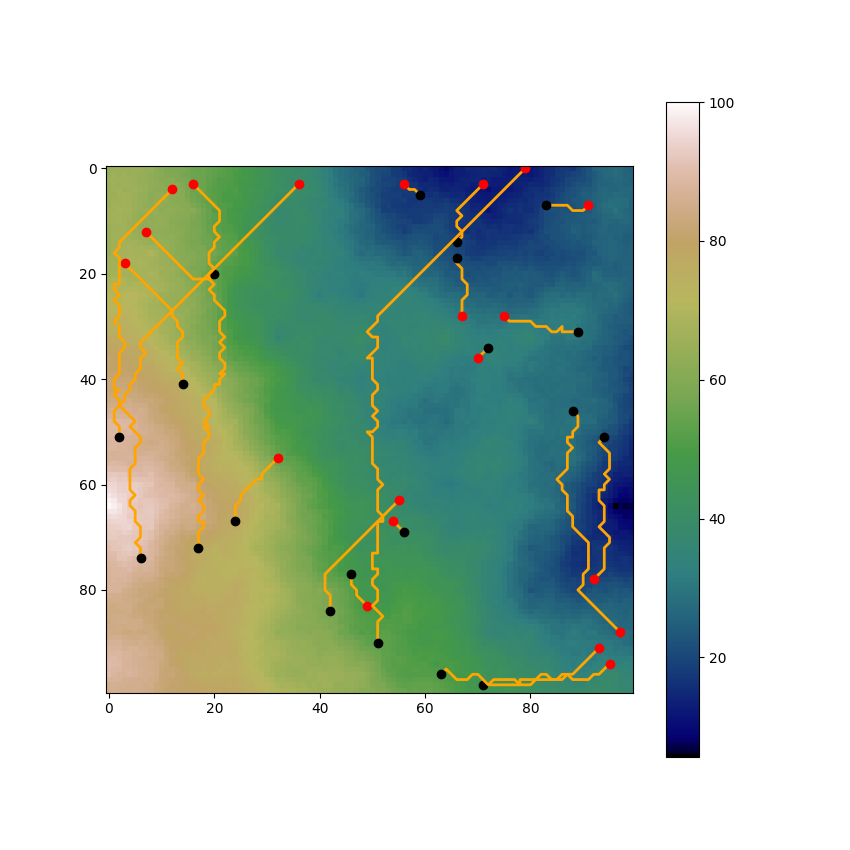
\includegraphics[width = 1.0\columnwidth]{data/mean_paths/100x100/20.png}
			\caption*{20 роботов}
			\end{subfigure}
			&
			\begin{subfigure}{0.5\linewidth}
				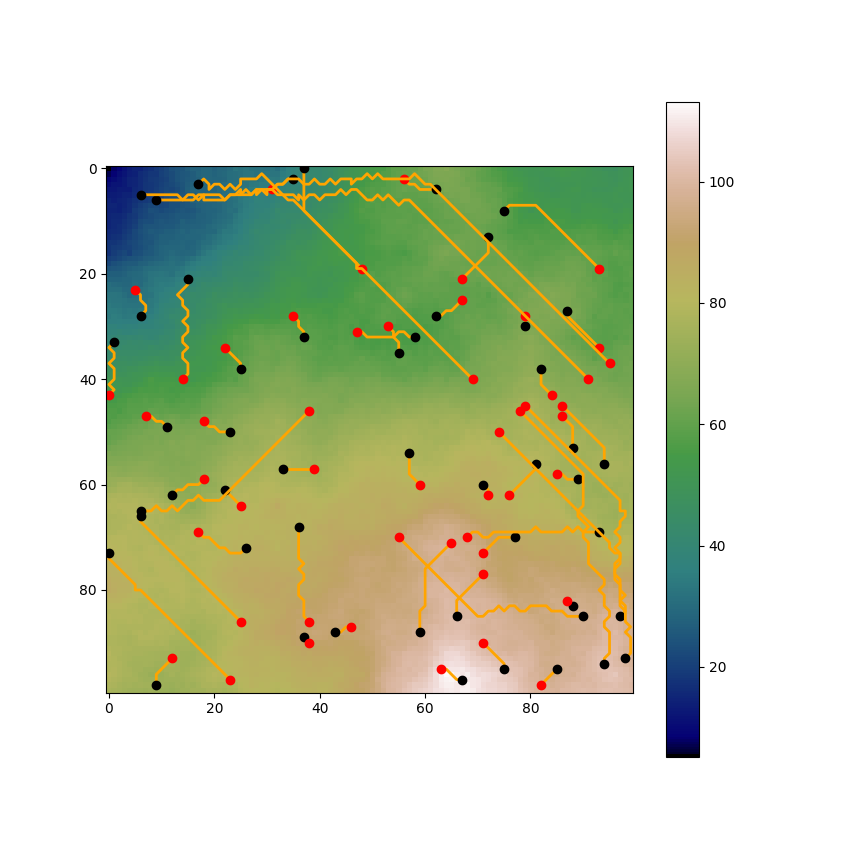
\includegraphics[width = 1.0\columnwidth]{data/mean_paths/100x100/50.png}
			\caption*{50 роботов}
			\end{subfigure}
        \end{tabular}
        \caption*{Размер карты: 100x100}
	\end{table}

	\begin{table}[H]
		\begin{tabular}{c c}
			\begin{subfigure}{0.5\linewidth}
				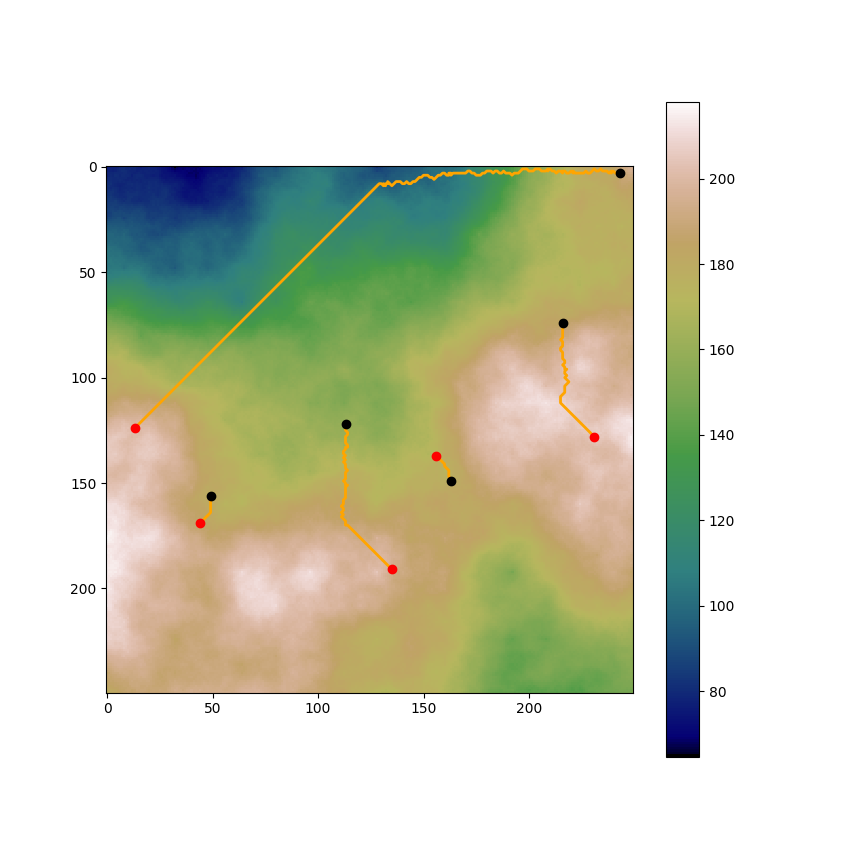
\includegraphics[width = 1.0\columnwidth]{data/mean_paths/250x250/5.png}
			\caption*{5 роботов}
			\end{subfigure}
			&
			\begin{subfigure}{0.5\linewidth}
				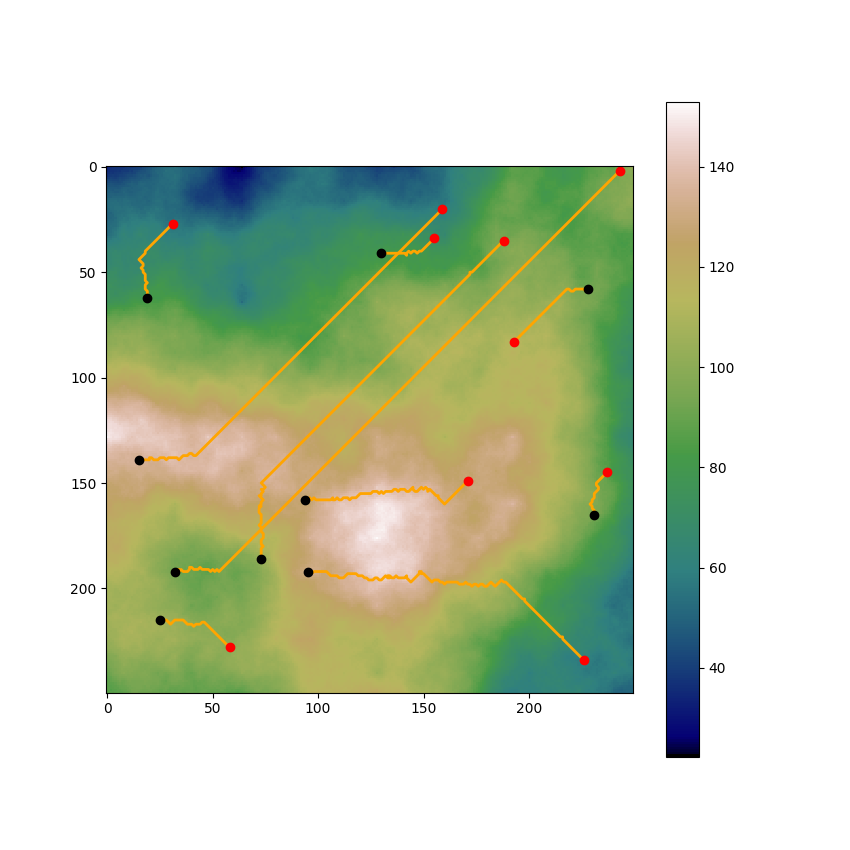
\includegraphics[width = 1.0\columnwidth]{data/mean_paths/250x250/10.png}
			\caption*{10 роботов}
			\end{subfigure}
			\\
            \begin{subfigure}{0.5\linewidth}
				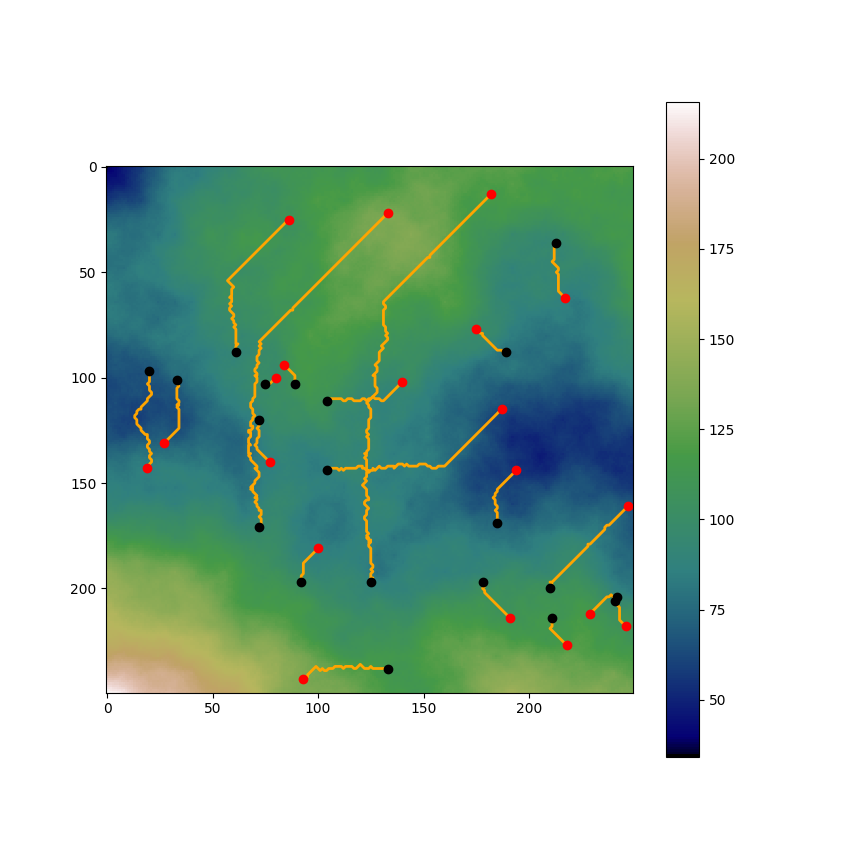
\includegraphics[width = 1.0\columnwidth]{data/mean_paths/250x250/20.png}
			\caption*{20 роботов}
			\end{subfigure}
			&
			\begin{subfigure}{0.5\linewidth}
				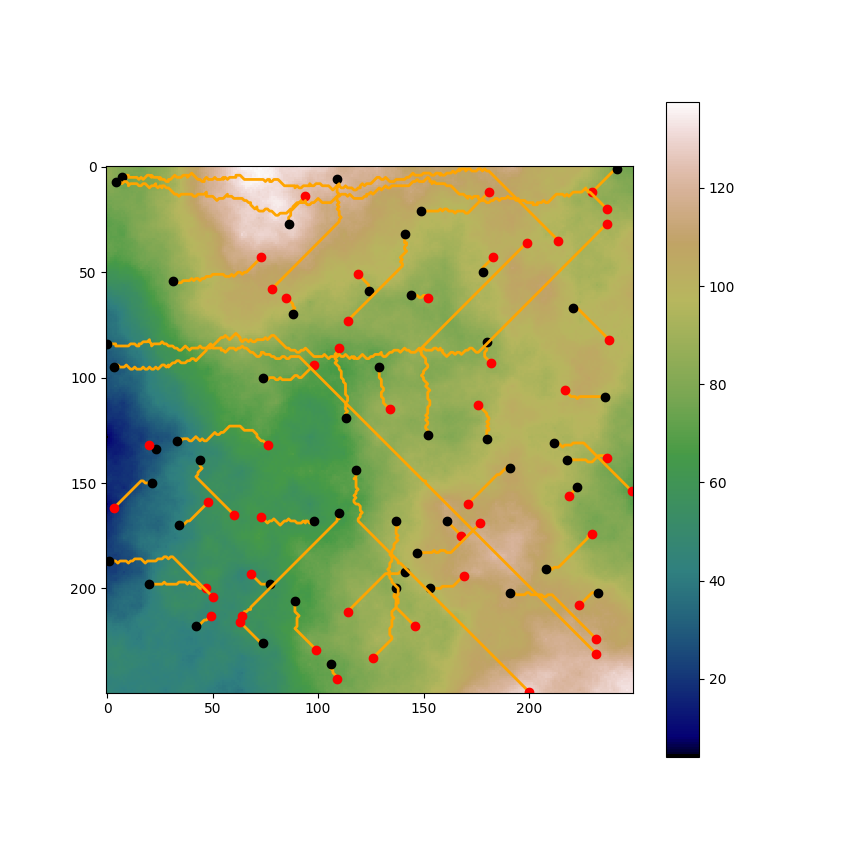
\includegraphics[width = 1.0\columnwidth]{data/mean_paths/250x250/50.png}
			\caption*{50 роботов}
			\end{subfigure}
        \end{tabular}
        \caption*{Размер карты: 250x250}
	\end{table}

	\begin{table}[H]
		\begin{tabular}{c c}
			\begin{subfigure}{0.5\linewidth}
				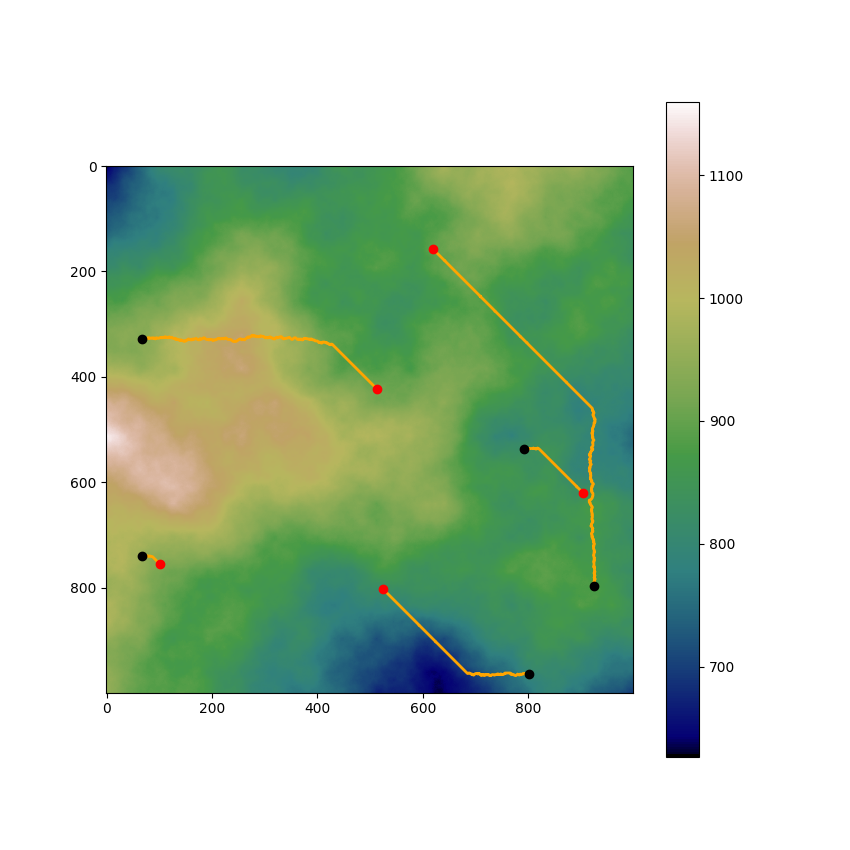
\includegraphics[width = 1.0\columnwidth]{data/mean_paths/1000x1000/5.png}
			\caption*{5 роботов}
			\end{subfigure}
			&
			\begin{subfigure}{0.5\linewidth}
				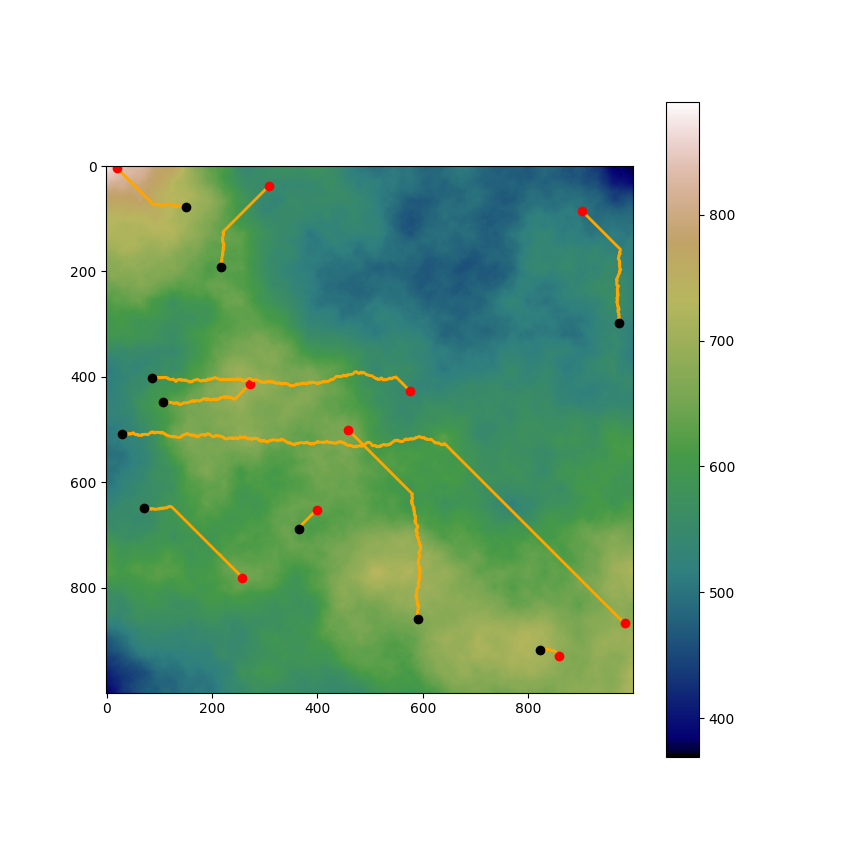
\includegraphics[width = 1.0\columnwidth]{data/mean_paths/1000x1000/10.png}
			\caption*{10 роботов}
			\end{subfigure}
			\\
            \begin{subfigure}{0.5\linewidth}
				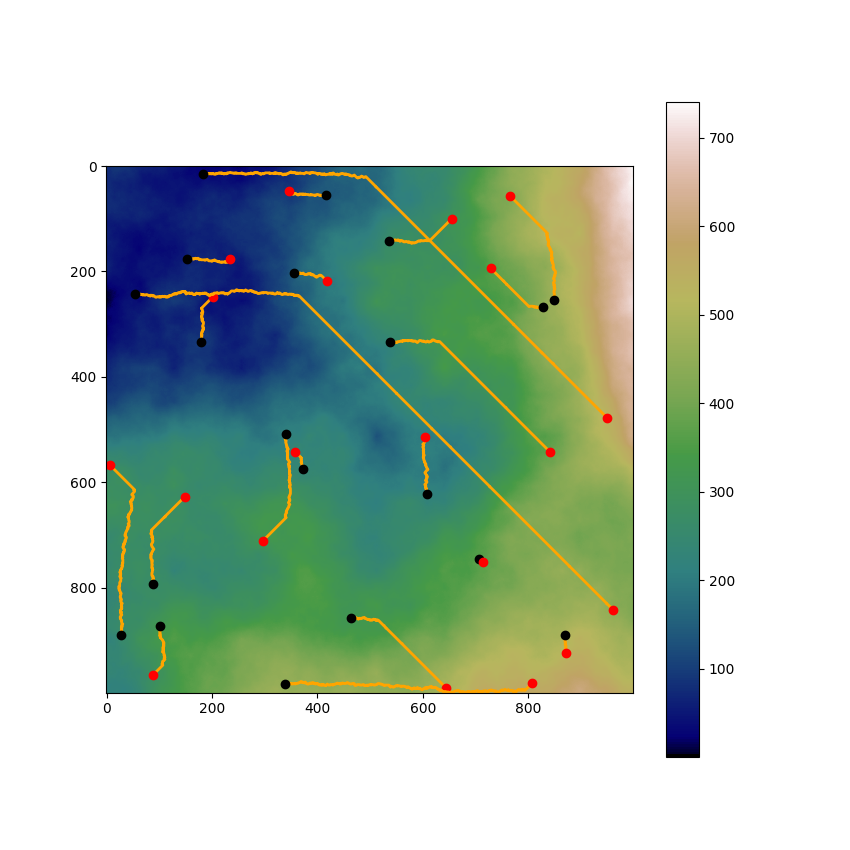
\includegraphics[width = 1.0\columnwidth]{data/mean_paths/1000x1000/20.png}
			\caption*{20 роботов}
			\end{subfigure}
			&
			\begin{subfigure}{0.5\linewidth}
				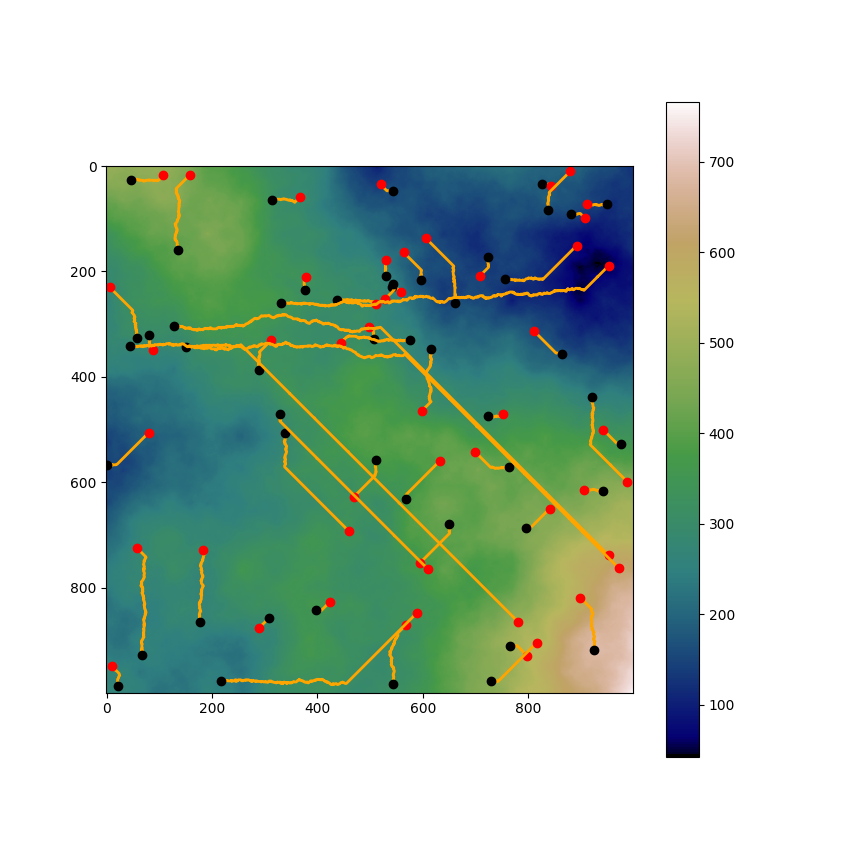
\includegraphics[width = 1.0\columnwidth]{data/mean_paths/1000x1000/50.png}
			\caption*{50 роботов}
			\end{subfigure}
        \end{tabular}
        \caption*{Размер карты: 1000x1000}
	\end{table}

\end{document}
